\documentclass[a4paper,12pt,twoside]{article}
\usepackage[left=1in,right=1in,top=1in,bottom=1in]{geometry}

\usepackage{xeCJK}
\setCJKmainfont{Songti TC}
\setCJKfamilyfont{kai}{Songti TC}
\newcommand{\kai}{\CJKfamily{kai}} % 用 \kai{使用楷書}

\usepackage{lmodern}
\usepackage{titling}
\usepackage{titlesec}
\usepackage{graphicx}
\usepackage{float}
\usepackage{amsmath, amsthm, amssymb, amsfonts, mathrsfs}
\usepackage{upgreek} % 直立的希臘字母

\usepackage[shortlabels]{enumitem}
\usepackage{setspace}
\renewcommand{\baselinestretch}{1.5}
\usepackage[colorlinks]{hyperref}
\usepackage{fancyvrb}
\usepackage{fancyhdr}
\usepackage{multicol}
\usepackage{caption}
\usepackage{listings}
\usepackage{bm}
\usepackage{bbm} % for \mathbbm{1} (indicator function)
\usepackage{centernot}
\usepackage{mdframed}
\usepackage{tikz}
\usetikzlibrary{patterns, arrows.meta, positioning}
\usepackage[nameinlink, capitalise]{cleveref}
\usepackage{diagbox}
\usepackage{booktabs}
\usepackage{multirow,array}
\usepackage{tabularx}
\usepackage{mathtools}
\usepackage{indentfirst} % 首段 indent
\setlength{\parindent}{2em}
\usepackage{cancel} % 數學式子畫線槓掉
\newcommand\mcancel[2][red]{\setbox0=\hbox{$#2$}%
\rlap{\raisebox{.45\ht0}{\textcolor{#1}{\rule{\wd0}{1pt}}}}#2}
\usepackage{datetime2}

\AtBeginDocument{%
 \setlength{\abovedisplayskip}{6pt}
 \setlength{\belowdisplayskip}{6pt}
 \setlength{\abovedisplayshortskip}{4pt}
 \setlength{\belowdisplayshortskip}{4pt}
}

\definecolor{codegreen}{rgb}{0,0.6,0}
\definecolor{codegray}{rgb}{0.5,0.5,0.5}
\definecolor{codepurple}{rgb}{0.58,0,0.82}
\definecolor{backcolour}{rgb}{0.95,0.95,0.92}

\lstdefinestyle{mystyle}{
 backgroundcolor=\color{backcolour},
 commentstyle=\color{codegreen},
 keywordstyle=\color{magenta},
 numberstyle=\tiny\color{codegray},
 stringstyle=\color{codepurple},
 basicstyle=\ttfamily\footnotesize,
 breakatwhitespace=false,
 breaklines=true,
 captionpos=b,
 keepspaces=true,
 numbers=left,
 numbersep=5pt,
 showspaces=false,
 showstringspaces=false,
 showtabs=false,
 tabsize=2
}
\lstset{style=mystyle}

\hypersetup{citecolor=blue, linkcolor=blue, urlcolor=blue}

\DeclareMathOperator{\supp}{supp}
\DeclareMathOperator{\skewness}{Skewness}
\DeclareMathOperator{\DU}{D-U}
\DeclareMathOperator{\CU}{C-U}
\DeclareMathOperator{\Geo}{Geo}
\DeclareMathOperator{\Pois}{Pois}
\DeclareMathOperator{\Gam}{Gam}
\DeclareMathOperator{\LN}{LogN}
\DeclareMathOperator{\cov}{Cov}
\DeclareMathOperator*{\argmax}{arg\,max}
\DeclareMathOperator*{\argmin}{arg\,min}
\DeclareMathOperator{\re}{Re}
\DeclareMathOperator{\im}{Im}

\newcommand{\N}{\mathbb{N}}
\newcommand{\Z}{\mathbb{Z}}
\newcommand{\Q}{\mathbb{Q}}
\newcommand{\R}{\mathbb{R}}
\newcommand{\C}{\mathbb{C}}
\newcommand{\G}{\mathcal{G}}
\newcommand{\mP}{\mathbb{P}}
\newcommand{\F}{\mathcal{F}}
\newcommand{\B}{\mathcal{B}}
\newcommand{\1}{\mathbbm{1}}
\newcommand{\Poi}{\text{Poi}}
\newcommand{\Var}{\text{Var}}
\newcommand{\as}{\text{a.s.}}
\newcommand{\vect}[1]{\boldsymbol{\mathbf{#1}}}
\newcommand{\paren}[1]{\left({#1}\right)}
\newcommand{\brk}[1]{\left[{#1}\right]}
\newcommand{\curl}[1]{\left\{{#1}\right\}}
\renewcommand{\lambda}{\lambdaup}

\theoremstyle{definition} % 定理環境 style 改用正體
\newtheorem{theorem}{定理}
\newtheorem{definition}{定義}
\newtheorem*{definition*}{定義}
\newtheorem{example}{例子}
\newtheorem{exercise}{練習}
\newtheorem{corollary}{推論}
\newtheorem{property}{性質}
\newtheorem{prop}{命題}
\newtheorem{lemma}{引理}
\newtheorem{problem}{問題}
\newtheorem*{remark}{註}

\renewcommand{\figurename}{圖}
\renewcommand{\tablename}{表}

\DeclareMathOperator{\var}{Var}
\DeclareMathOperator{\corr}{corr}
\DeclareMathOperator{\rank}{rank}
\DeclareMathOperator{\MSE}{MSE}
\DeclareMathOperator{\SSE}{SSE}
\DeclareMathOperator{\SST}{SST}
\DeclareMathOperator{\SSR}{SSR}
\DeclareMathOperator{\sgn}{sign}
\DeclareMathOperator{\alt}{Alt}
\DeclareMathOperator{\adj}{adj}
\DeclareMathOperator{\curlOp}{curl}
\DeclareMathOperator{\spn}{span}
\DeclareMathOperator{\sse}{SSE}
\DeclareMathOperator{\tr}{tr}

\newcommand{\ep}{\varepsilon}
\newcommand{\p}{\partial}
\newcommand{\abs}[1]{\left|#1\right|}
\newcommand\norm[1]{\left\lVert#1\right\rVert}
\newcommand{\innerprod}[1]{\langle#1\rangle}
\newcommand{\ds}{\displaystyle}
\newcommand{\blank}{\rule[-1mm]{1.5cm}{0.1mm}}
\newcommand{\dint}{\displaystyle\int}
\renewcommand{\bar}{\overline}

\newtheoremstyle{remark}{}{}{}{}{\bfseries\sffamily}{.}{.5em}{#1}
\theoremstyle{remark}

\newtheorem*{remark*}{\textit{Remark}}
\newtheorem*{solution*}{解}

\AtEndEnvironment{solution*}{\hfill$\square$}
\newtheorem*{hint*}{Hint}


\newcommand{\redtext}[1]{{\color{red} #1}}
\newcommand{\bluetext}[1]{{\color{blue} #1}}

\fancypagestyle{firstpage}{
  \fancyhf{}
  \fancyhead[R]{\small《高中數學實驗教材》第 3 冊（自然組）}
  \fancyhead[L]{\small 第 2 章\quad 直觀幾何與三角函數}
  \fancyfoot[C]{\thepage}
}

\pagestyle{fancy}
\setlength{\headheight}{14pt}
\renewcommand{\headrulewidth}{0.5pt}
\renewcommand{\footrulewidth}{0pt}
\fancyhead{}
\fancyhead[LE]{\small 《高中數學實驗教材》第三冊（自然組）}
\fancyhead[RO]{\small 第二章\quad 直觀幾何與三角函數}
\fancyfoot[C]{\thepage}

\title{\LARGE\textbf{《高中數學實驗教材》第三冊（自然組）}\\[0.5em] \Large\textbf{第二章\quad 直觀幾何與三角函數}}
\author{\textbf{高中數學實驗教材編輯小組}\quad 編著}
\date{民國六十四年（1975）再版}

\begin{document}

\maketitle
\thispagestyle{firstpage}

% ==========================================
% 掃描檔勘誤、文字校訂與疑難處說明（依規則整理於目錄之前）
% ==========================================
\section*{【說明】第二章掃描檔勘誤、疑難處與文義校訂表}
\addcontentsline{toc}{section}{【說明】第二章掃描檔勘誤、疑難處與文義校訂表}
\label{sec:errata_notes_b3_ch2}

本章依據 1975 年再版《高中數學實驗教材 第三冊（自然組）》（高二上）第二章「直觀幾何與三角函數」掃描原件完整轉錄為 \LaTeX{} 格式。為忠實反映教材原始內容並兼顧排版品質與嚴謹性，依作業規範將掃描檔中出現之印刷訛誤、符號缺漏、字模損毀、歷史印記雜訊及文義疑難處詳細考證彙整於下表。讀者可點擊表格中之章節連結直接跳至正文對應位置：

\begin{table}[H]
\centering
\small
\renewcommand{\arraystretch}{1.35}
\begin{tabularx}{\textwidth}{|p{3.2cm}|p{3.8cm}|X|}
\hline
\textbf{章節位置} & \textbf{掃描檔原始現象 / 誤植} & \textbf{考證說明與校訂處理} \\ \hline

\hyperref[note:b3-ch2-p37-fig2-25-2]{§ 2-2 頁 37 圖 2-25-2 說明} & 
「(此圖 $-\frac{3\pi}{2} < \theta < \pi$; $x<0, y>0$)」 & 
右端「$\pi$」實為「$-\pi$」（順時針負角旋轉對應第二象限實為 $-\frac{3\pi}{2} < \theta < -\pi$）。正文照原印字樣錄入並備註說明。 \\ \hline

\hyperref[note:b3-ch2-p41-ex4-typo]{§ 2-2 頁 41 例 4 題幹} & 
「已知 $\alpha = 1230^\circ$，求 $\sin\alpha, \cos\alpha, \text{tara }\alpha$ 之值」 & 
「tara $\alpha$」顯為「$\tan\alpha$」之印刷訛字。正文照原印字樣錄入並註記。 \\ \hline

\hyperref[note:b3-ch2-p41-ref-fig31]{§ 2-2 頁 41 例 4 末行插圖} & 
「則終邊 $\mathbf{r}_2$ 落在第二象限 $\mathrm{II}$（如圖 2-31）」 & 
圖 2-31 實為前文割線函數圖形，本題對應之旋轉終邊圖印於次頁圖 2-32。正文保留原書字樣。 \\ \hline

\hyperref[note:b3-ch2-p60-ex12-data]{§ 2-5 頁 60 例 12 題幹} & 
「$b = 1000\sqrt{6}$ 公尺」 & 
解文中計算代入數值為 $100\sqrt{6}$ 公尺，算得結果 $467.5$ 公尺，題幹數值多植一零。正文照原印字樣錄入並備註說明。 \\ \hline

\hyperref[note:b3-ch2-p61-ex13-sir]{§ 2-5 頁 61 例 13 算式} & 
「$a\text{ sir}(\frac{\pi}{2} - 28^\circ 40')$」 & 
英文正弦函數記號「$\sin$」誤植為「sir」。正文照原刊字樣錄入並註記。 \\ \hline

\hyperref[note:b3-ch2-p66-homework16-deg]{§ 2-5 頁 66 作業 16} & 
「$\angle CAB = 120$」 & 
題幹漏印度數符號「$^\circ$」，實為 $120^\circ$。正文照原印樣式錄入並備註說明。 \\ \hline

\end{tabularx}
\end{table}

\clearpage
\tableofcontents
\newpage

% =========================================================================
% 《高中數學實驗教材》第三冊（自然組）
% 第二章 直觀幾何與三角函數
% =========================================================================

\section{直觀幾何與三角函數}
\label{sec:b3-ch2}

\begin{center}
\begin{minipage}{0.65\textwidth}
\begin{itemize}[leftmargin=2em, itemsep=0.3em]
  \item[§2-1] 有向線段與有向角
  \begin{itemize}[leftmargin=2em, itemsep=0.2em]
    \item[甲、] 有向角
    \item[乙、] 無向角
    \item[丙、] 有向角的推廣
    \item[丁、] 角的記號
    \item[戊、] 同界角
    \item[己、] 角度的單位
    \item[庚、] 扇形
  \end{itemize}
  \item[§2-2] 三角函數的定義
  \begin{itemize}[leftmargin=2em, itemsep=0.2em]
    \item[甲、] 銳角的三角函數
    \item[乙、] 三角函數
  \end{itemize}
  \item[§2-3] 一些簡易的恒等式
  \item[§2-4] 一些幾何上量的定理
  \begin{itemize}[leftmargin=2em, itemsep=0.2em]
    \item[甲、] 畢氏定理的推廣
    \item[乙、] 三角形之面積與邊長
  \end{itemize}
  \item[§2-5] 三角測量
\end{itemize}
\end{minipage}
\end{center}

\begin{center}
$* \qquad * \qquad * \qquad * \qquad *$
\end{center}

國中教科書上已學過直線、三角形、平行四邊形與圓等的一些幾何圖形的基本性質，同時也提過利用銳角三角函數去作一些簡易的測量.

我們假定對那些學過的東西已相當熟悉，而要利用本章的篇幅進一步作更細膩的申述，以方便以後的用途. 同時利用這些剛發展出來的三角函數的工具應用到測量上去，趁此也再一次說明了第一章中所提實際問題、幾何與代數間的轉化關係.

我們將討論一般廣義角的三角函數來代替國中考慮的特殊情形：銳角的三角函數. 這樣一來我們才能廣泛推展三角函數間的運算.

\subsection{有向線段與有向角}
\label{subsec:b3-2-1}

\subsubsection*{甲、有向角}

有甲乙兩地，由甲地引到乙地的\textbf{有向線段}，可以看成是乙地相對於甲地位置的一種描寫. 一個有向線段依它的「始點」「方向」「長度」而決定，比如，「自甲地向東北方走 5 公里」此時始點是甲地，方向是東北向，長度是 5 公里. 這樣便得到乙地，且描寫出來乙地相對於甲地的位置.

\begin{figure}[H]
\centering
\begin{tikzpicture}[>=stealth, scale=0.9, font=\small]
  \coordinate (A) at (0, 0);
  \coordinate (B) at (3.5, 2.5);
  \draw[->, very thick] (A) -- (B) node[midway, above left, sloped] {5公里};
  \fill (A) circle (2pt) node[below left] {甲地};
  \fill (B) circle (2pt) node[right] {乙地};
\end{tikzpicture}
\caption{有向線段}
\label{fig:b3-fig2-1}
\end{figure}

同樣地把上述「相對位置」的考慮改成「相對方位」的考慮，我們將得到所謂有向角.

地理或航海上，我們慣於使用「方位」的字眼來代替「方向」. 設平面上有甲、乙兩種方位，若已知甲方位，欲求乙方位，我們便須知道乙方位相對於甲方位的「相對方位」或「方位差」，例如：乙方 arbitrary 乃由甲方位按逆時針方向旋轉 $120^\circ$ 而得. 比照於有向線段，我們引進來\textbf{有向角}的觀念，它由下列三個因素組成：

「始邊」「旋轉方向」「旋轉量」

就如在上述例子中，始邊是甲方位，旋轉方向是逆時針方向，旋轉量則為 $120^\circ$.

\begin{figure}[H]
\centering
\begin{tikzpicture}[>=stealth, scale=0.9, font=\small]
  \coordinate (O) at (0, 0);
  \draw[->, very thick] (O) -- (0, 3) node[right] {乙方位};
  \draw[->, very thick] (O) -- (120:3) node[above left] {甲方位};
  \draw[->, thick] (0.8, 0) arc (0:120:0.8) node[midway, above right] {$120^\circ$};
  \fill (O) circle (1.5pt);
\end{tikzpicture}
\caption{有向角方位示意}
\label{fig:b3-fig2-2}
\end{figure}

平面上的有向角，其可能的旋轉方向只有逆時針與順時針兩個方向，我們用正負向來區別它們：規定逆時針旋轉便是正向，順時針旋轉便是負向，並據此將正號或負號記在旋轉量之前，稱為有向角的角度. 換句話說，有向角的旋轉方向及旋轉量合併起來，稱為有向角的角度. 像上例的有向角，角度為 $+120^\circ$，或簡記為 $120^\circ$（但負號不能省略）. 又如圖 2-3：

\begin{figure}[H]
\centering
\begin{minipage}{0.48\textwidth}
\centering
\begin{tikzpicture}[>=stealth, scale=0.9, font=\small]
  \coordinate (O) at (0, 0);
  \draw[->, very thick] (O) -- (60:2.5) node[above] {乙方位};
  \draw[->, very thick] (O) -- (120:2.5) node[above] {甲方位};
  \draw[->, thick] (120:0.9) arc (120:60:0.9) node[midway, below] {$-60^\circ$};
\end{tikzpicture}
\end{minipage}
\hfill
\begin{minipage}{0.48\textwidth}
\centering
\begin{tikzpicture}[>=stealth, scale=0.9, font=\small]
  \coordinate (O) at (0, 0);
  \draw[->, very thick] (O) -- (0, 2.5) node[right] {甲方位};
  \draw[->, very thick] (O) -- (120:2.5) node[above left] {乙方位};
  \draw[->, thick] (0.8, 0) arc (0:-240:0.8) node[midway, below] {$-240^\circ$};
\end{tikzpicture}
\end{minipage}
\caption{負向旋轉之有向角}
\label{fig:b3-fig2-3}
\end{figure}

左圖有向角之角度記為 $-60^\circ$，右圖則記以 $-240^\circ$.

這樣一個有向角可由它的「始邊」與「角度」來決定，另一方面，也可由它的「始邊」「旋轉方向」「終邊」來決定.（即以「終邊」代替上述的「旋轉量」）. 例如圖 2-4 中，若確知始邊為正北方位，終邊為東南方位，而旋轉方向為負向（即順時針方向），則旋轉量知為 $135^\circ$. 反過來，若確知始邊為正北，旋轉方向為負向，而旋轉量為 $135^\circ$，則終邊知為東南方位.

\begin{figure}[H]
\centering
\begin{tikzpicture}[>=stealth, scale=0.9, font=\small]
  \draw[->, very thick] (0, 0) -- (0, 3) node[above] {$N$ 正北方位};
  \draw[->, very thick] (0, 0) -- (45:3) node[above right] {東南方位 $SE$};
  \draw[->, thick] (0, 1) arc (90:-45:1) node[midway, right] {$-135^\circ$};
  \draw[->, thick, dashed] (0, 1.4) arc (90:315:1.4) node[midway, left] {$225^\circ$};
\end{tikzpicture}
\caption{方位角旋轉對照}
\label{fig:b3-fig2-4}
\end{figure}

\subsubsection*{乙、無向角}

國中講過的「角」，其實就是將上述的有向角，不分其兩邊誰始誰終，只考慮角的兩邊，也因此不分其旋轉方向是正是負，只管旋轉後留下的痕跡. 這樣的角，在必要區別時，我們特稱為\textbf{無向角}，平常仍沿稱為角. 無向角的角度便是它張角的大小，永遠不為負值.

圖 2-5 左側兩個有向角都對應到同一個畫在右側的無向角.

\begin{figure}[H]
\centering
\begin{tikzpicture}[>=stealth, scale=0.85, font=\small]
  % Left 1: +120
  \coordinate (O1) at (0, 0);
  \draw[->, thick] (O1) -- (2, -1) node[right] {始邊};
  \draw[->, thick] (O1) -- (0.5, 2) node[above] {終邊};
  \draw[->, thick] ($(O1)+(2,-1)!0.4!(O1)$) arc (-26.5:76:0.8) node[midway, above left] {$120^\circ$};

  \node at (2.5, 0.5) {與};

  % Left 2: -120
  \coordinate (O2) at (4, 0);
  \draw[->, thick] (O2) -- (4.5, 2) node[above] {始邊};
  \draw[->, thick] (O2) -- (6, -1) node[right] {終邊};
  \draw[->, thick] (4.5, 0.8) arc (76:-26.5:0.8) node[midway, right] {$-120^\circ$};

  \draw[->, very thick] (6.8, 0.5) -- (7.8, 0.5);

  % Right: Undirected 120
  \coordinate (O3) at (9.5, 0);
  \draw[thick] (O3) -- (11.5, -1);
  \draw[thick] (O3) -- (10, 2);
  \draw (10.3, -0.4) arc (-26.5:76:0.8) node[midway, above right] {$120^\circ$};
\end{tikzpicture}
\caption{有向角與無向角之對應 (一)}
\label{fig:b3-fig2-5-1}
\end{figure}

\begin{figure}[H]
\centering
\begin{tikzpicture}[>=stealth, scale=0.85, font=\small]
  % Left 1: -240
  \coordinate (O1) at (0, 0);
  \draw[->, thick] (O1) -- (1.8, -1.2) node[right] {始邊};
  \draw[->, thick] (O1) -- (0.5, 2) node[above] {終邊};
  \draw[->, thick] (0.8, -0.5) arc (-33:247:0.9) node[midway, left] {$-240^\circ$};

  \node at (2.5, 0.5) {與};

  % Left 2: +240
  \coordinate (O2) at (4, 0);
  \draw[->, thick] (O2) -- (4.5, 2) node[above] {始邊};
  \draw[->, thick] (O2) -- (5.8, -1.2) node[right] {終邊};
  \draw[->, thick] (4.5, 0.8) arc (76:307:0.9) node[midway, left] {$240^\circ$};

  \draw[->, very thick] (6.8, 0.5) -- (7.8, 0.5);

  % Right: Undirected 240
  \coordinate (O3) at (9.5, 0);
  \draw[thick] (O3) -- (11.3, -1.2);
  \draw[thick] (O3) -- (10, 2);
  \draw (10.3, -0.4) arc (-33:247:0.9) node[midway, left] {$240^\circ$};
\end{tikzpicture}
\caption{有向角與無向角之對應 (二)}
\label{fig:b3-fig2-5-2}
\end{figure}

給了兩邊，我們取它所夾的兩個角中的較小的那一個無向角，稱為這兩邊的\textbf{夾角}.〔當這邊所代表的兩條射線方向正好相反時，必須再另外指定所取的夾角是哪一個無向角〕這兩邊則稱為這個無向角的兩個夾邊.

\subsubsection*{丙、有向角的推廣}

在第一章我們提過，若約定一個基準點 $O$，則空間（或平面上）任一點 $P$ 的位置，可由其相應的有向線段 $\vec{OP}$ 來決定. 同樣我們約定一基準方位 $\mathbf{r}_0$，〔習慣上，作圖時取之為地圖上的東向，這相當於慣常我們沿一座標系 $(O; X, Y)$ 繪出的 $OX$ 軸方向〕，使得任一方位 $\mathbf{r}$ 皆可由 $\mathbf{r}_0$ 繞到 $\mathbf{r}$ 的有向角之角度確定，如給定 $120^\circ$（或 $-240^\circ$）便可確定的正確方位.

\begin{figure}[H]
\centering
\begin{tikzpicture}[>=stealth, scale=0.9, font=\small]
  \coordinate (O) at (0, 0);
  \draw[->, very thick] (O) -- (3.5, 0) node[right] {$X$（基準方位 $\mathbf{r}_0$）};
  \draw[->, very thick] (O) -- (120:3) node[above left] {$\mathbf{r}$};
  \draw[->, thick] (0.8, 0) arc (0:120:0.8) node[midway, above right] {$120^\circ$};
  \draw[->, thick, dashed] (1.1, 0) arc (0:-240:1.1) node[midway, below] {$-240^\circ$};
  \fill (O) circle (1.5pt) node[below left] {$O$};
\end{tikzpicture}
\caption{基準方位與角度定位}
\label{fig:b3-fig2-6}
\end{figure}

如果只一味要考慮「相對方位」或「方位差」，上述有向角的定義便已妥善無虞. 但以後我們將會見到我們有需要不把有向角限制在 $-360^\circ$ 到 $+360^\circ$ 之間. 很多時候，雖然我們繞了 $360^\circ$（或 $-360^\circ$）又回到原來的方位，但有些相關的狀況卻已改變. 若把有向角看成是方位的旋轉本身，那麼一個磨穀的石磨仔旋轉一百圈後，回到原來的方位，與它從來不曾旋轉明顯有著區別. 為了把這種區別顯示出來，我們要推廣有向角的定義：

一個\textbf{廣義有向角}可以看成是一條射線的“單向”轉動（單向指在逆時針或順時針中取定一方向）其度量可由其旋轉方向及旋轉量來給定. 與（狹義）有向角的情形一樣，它的度量稱為廣義有向角的角度，它可以是任意一個實數.

例如它可以是 $+780^\circ$ 或 $-510^\circ$，前者表示一條射線沿逆時針方向繞整整兩圈後接著又繞了 $60^\circ$ 的一個旋轉.（因 $780^\circ = 2\times 360^\circ + 60^\circ$）. 後者表示一條射線沿順時針方向整整繞了一圈後，接著又繼續繞了 $150^\circ$ 角度的旋轉（因 $-510^\circ = (-1)\times 360^\circ + (-150^\circ)$）.

\begin{figure}[H]
\centering
\begin{minipage}{0.48\textwidth}
\centering
\begin{tikzpicture}[>=stealth, scale=0.9, font=\small]
  \coordinate (O) at (0, 0);
  \draw[->, very thick] (O) -- (60:2.5) node[above] {始邊};
  \draw[->, very thick] (O) -- (120:2.5) node[above] {終邊};
  \draw[->, thick, domain=0:780, samples=200, variable=\t]
    plot ({0.25 + 0.0008*\t)*cos(\t+60)}, {(0.25 + 0.0008*\t)*sin(\t+60)});
  \node[below] at (0, -0.9) {$+780^\circ$};
  \node[above] at (-0.2, 0.7) {$60^\circ$};
\end{tikzpicture}
\caption{$+780^\circ$ 廣義旋轉角}
\label{fig:b3-fig2-8-1}
\end{minipage}
\hfill
\begin{minipage}{0.48\textwidth}
\centering
\begin{tikzpicture}[>=stealth, scale=0.9, font=\small]
  \coordinate (O) at (0, 0);
  \draw[->, very thick] (O) -- (60:2.5) node[above] {始邊};
  \draw[->, very thick] (O) -- (270:2) node[below] {終邊};
  \draw[->, thick, domain=0:510, samples=200, variable=\t]
    plot ({0.25 + 0.001*\t)*cos(60-\t)}, {(0.25 + 0.001*\t)*sin(60-\t)});
  \node[right] at (0.8, -0.4) {$-510^\circ$};
  \node[above left] at (0.2, 0.4) {$210^\circ$};
\end{tikzpicture}
\caption{$-510^\circ$ 廣義旋轉角}
\label{fig:b3-fig2-8-2}
\end{minipage}
\end{figure}

由於前述的有向角只不過是廣義有向角的特殊情形，（換句話說，有向角只不過是角度介於 $0^\circ$ 與 $360^\circ$ 之間的廣義有向角）. 以後我們可以單單考慮廣義有向角，而把它略稱為有向角.

不管是（廣義）有向角或無向角，以後我們都沿依習慣，通稱為\textbf{角}. 必要區別時，我們再予明言.

\subsubsection*{丁、角的記號}

一個（廣義）有向角，角度 $\theta$（含旋轉方向與旋轉量）與始邊 $\mathbf{r}_1$ 確定後，這個有向角本身也就確定. 有時為了特別要表明始終邊 $\mathbf{r}_1, \mathbf{r}_2$ 的位置，把這個有向角記成 $\angle(\theta; \mathbf{r}_1, \mathbf{r}_2)$，方便上簡記為 $\angle\theta$. 注意這時 $\theta$ 可正可負，例如圖 2-9-1 中 $\theta = -35^\circ$.

\begin{figure}[H]
\centering
\begin{minipage}{0.48\textwidth}
\centering
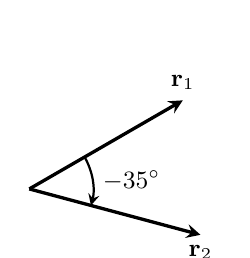
\begin{tikzpicture}[>=stealth, scale=0.9, font=\small]
  \coordinate (O) at (0, 0);
  \draw[->, very thick] (O) -- (30:2.5) node[above] {$\mathbf{r}_1$};
  \draw[->, very thick] (O) -- (-15:2.5) node[below] {$\mathbf{r}_2$};
  \draw[->, thick] (30:0.9) arc (30:-15:0.9) node[midway, right] {$-35^\circ$};
\end{tikzpicture}
\caption{$\angle(\theta; \mathbf{r}_1, \mathbf{r}_2)$ 有向角}
\label{fig:b3-fig2-9-1}
\end{minipage}
\hfill
\begin{minipage}{0.48\textwidth}
\centering
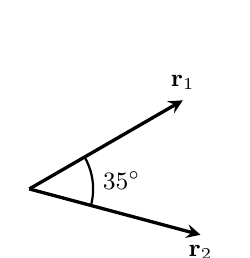
\begin{tikzpicture}[>=stealth, scale=0.9, font=\small]
  \coordinate (O) at (0, 0);
  \draw[->, very thick] (O) -- (30:2.5) node[above] {$\mathbf{r}_1$};
  \draw[->, very thick] (O) -- (-15:2.5) node[below] {$\mathbf{r}_2$};
  \draw[thick] (30:0.9) arc (30:-15:0.9) node[midway, right] {$35^\circ$};
\end{tikzpicture}
\caption{無向角記號}
\label{fig:b3-fig2-9-2}
\end{minipage}
\end{figure}

同樣，一個無向角，我們也記為 $\angle\theta$. 其中 $\theta$ 指它的角度，其值永不為負，例如圖 2-9-2 中 $\theta = 35^\circ$.

設 $\angle\theta$ 為 $\mathbf{r}_1, \mathbf{r}_2$ 的夾角，$\mathbf{r}_1, \mathbf{r}_2$ 上各有點 $B$ 與 $C$，且 $A$ 為 $\mathbf{r}_1$ 與 $\mathbf{r}_2$ 的公共端點（$A$ 稱為 $\angle\theta$ 的頂點），則 $\angle\theta$ 可記以
\[ \angle BAC \quad\text{或}\quad \angle CAB \]
以便於從圖上辨認，有時甚至略記為 $\angle A$. 即
\[ \angle\theta \equiv \angle BAC \equiv \angle CAB \equiv \angle A \]

我們列一個表來整理一下上述種種，它只是用來比較上述繁雜的陳述與規約，並不是要用來記憶.

\begin{figure}[H]
\centering
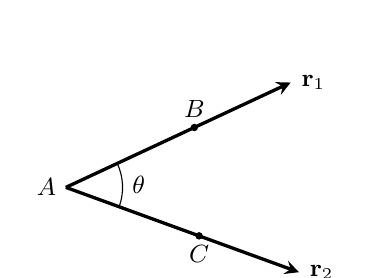
\begin{tikzpicture}[>=stealth, scale=0.9, font=\small]
  \coordinate (A) at (0, 0);
  \draw[->, very thick] (A) -- (25:3.5) node[right] {$\mathbf{r}_1$};
  \draw[->, very thick] (A) -- (-20:3.5) node[right] {$\mathbf{r}_2$};
  \fill (25:2) circle (1.5pt) node[above] {$B$};
  \fill (-20:2) circle (1.5pt) node[below] {$C$};
  \draw (25:0.8) arc (25:-20:0.8) node[midway, right] {$\theta$};
  \node[left] at (A) {$A$};
\end{tikzpicture}
\caption{夾角與頂點記號}
\label{fig:b3-fig2-10}
\end{figure}

\begin{table}[H]
\centering
\small
\renewcommand{\arraystretch}{1.25}
\begin{tabular}{|c|c|c|c|c|c|c|c|}
\hline
\multicolumn{2}{|c|}{} & 概念 & 記號 & 位置 & 起點；終點 & 方向 & 長度；範圍 \\ \hline
\multicolumn{2}{|c|}{有向線段} & 有向線段 & $\vec{AB}$ & $A, B$ 等 & $A; B$ &  & $\overline{AB},\; 0 \le \overline{AB}$ \\ \hline
\multirow{4}{*}{\shortstack{廣\\義\\有\\向\\角}} & 概念 & 有向角 & \multirow{2}{*}{\shortstack{$\angle(\theta; \mathbf{r}_1, \mathbf{r}_2)$\\或 $\angle\theta$}} & 方位 & 始邊；終邊 & 旋轉方向 & 角度；範圍 \\ \cline{2-3} \cline{5-8}
 & 記號 &  &  & $\mathbf{r}_1, \mathbf{r}_2$ 等 & $\mathbf{r}_1; \mathbf{r}_2$ &  & $\theta \in \mathbb{R}$ \\ \hline
\multirow{2}{*}{無向角} & 概念 & 無向角 & \multirow{2}{*}{\shortstack{$\angle\theta$\\$\angle A$\\$(\angle CAB, \angle BAC)$}} & 方位 & \shortstack{不分\\始邊；終邊} & \shortstack{不分旋轉方向\\只看旋轉留痕} & 角度；範圍 \\ \cline{2-3} \cline{5-8}
 & 記號 &  &  & $\mathbf{r}_1, \mathbf{r}_2$ 等 & \shortstack{$\mathbf{r}_1; \mathbf{r}_2$\\或 $\mathbf{r}_2; \mathbf{r}_1$} &  & \shortstack{$A, \angle A, \angle CAB, \angle BAC$\\$0 \le \theta < 360^\circ$} \\ \hline
\end{tabular}
\end{table}

但有向線段與有向角有一個基本的不能比照的地方：有了起點、終點便決定了一個有向線段. 但有了始邊、終邊，尚須給出逆或順時針方向才能決定出一個有向角. 因此，有向角的角度可能有正有負，依旋轉方向為逆或順時針方向而定；但有向線段則只須取其兩點間距，稱為長度，永遠不為負.

\begin{figure}[H]
\centering
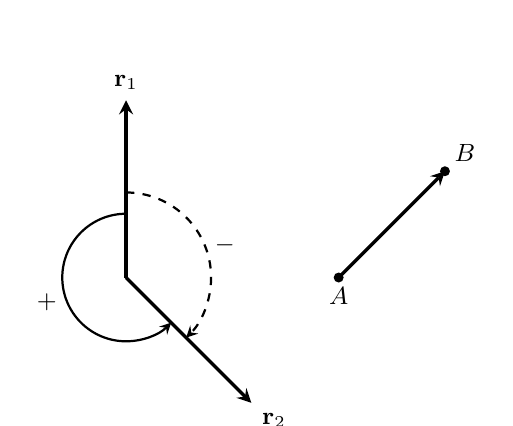
\begin{tikzpicture}[>=stealth, scale=0.9, font=\small]
  \coordinate (O) at (0, 0);
  \draw[->, very thick] (O) -- (0, 2.5) node[above] {$\mathbf{r}_1$};
  \draw[->, very thick] (O) -- (-45:2.5) node[below right] {$\mathbf{r}_2$};
  \draw[->, thick] (0, 0.9) arc (90:315:0.9) node[midway, left] {$+$};
  \draw[->, thick, dashed] (0, 1.2) arc (90:-45:1.2) node[midway, right] {$-$};
  
  \coordinate (A) at (3, 0);
  \coordinate (B) at (4.5, 1.5);
  \draw[->, very thick] (A) -- (B);
  \fill (A) circle (2pt) node[below] {$A$};
  \fill (B) circle (2pt) node[above right] {$B$};
\end{tikzpicture}
\caption{有向角與有向線段決定條件之差異}
\label{fig:b3-fig2-11}
\end{figure}

\subsubsection*{戊、同界角}

兩個（廣義）有向角，若具有相同的始邊與終邊，則稱它們互為\textbf{同界角}或\textbf{互為同界}. 例如圖 2-8 左圖中，轉 $+60^\circ$ 的角與轉 $+780^\circ$ 的角互為同界，而右圖中，轉 $+210^\circ$ 的角與轉 $-510^\circ$ 的角亦互為同界.

我們注意到兩個有向角 $\angle(\theta; \mathbf{r}_1, \mathbf{r}_2)$ 與 $\angle(\theta'; \mathbf{r}_1', \mathbf{r}_2')$ 互為同界角的一個充分必要條件是
\[ \mathbf{r}_1' = \mathbf{r}_1 \quad\text{且}\quad \theta' = \theta + 360^\circ \text{ 的整倍數} \]
要注意這個整倍數可以為正的倍數也可以為負的倍數. 例如圖 2-5 中角度分別為 $+120^\circ$ 與 $-240^\circ$ 的兩個（有向）角具有共同的始邊與終邊，它們是同界的. 這例子中
\[ -240^\circ = 120^\circ - 360^\circ \]
所取的倍數是 $-1$.

同樣，兩個無向角，若具有相同的兩個邊，也稱它們互為同界角或互為同界. 例如圖 2-5 中的兩個無向角，角度一為 $120^\circ$，一為 $240^\circ$，卻互為同界角. 注意這時候，兩個角度的差並不是 $360^\circ$ 的整倍數倒是這兩個角度的和等於 $360^\circ$. 這是一般的事實，換句話說，若兩個無向角 $\angle\theta$ 與 $\angle\theta'$ 互為同界角，則
\[ \theta + \theta' = 360^\circ \]

\subsubsection*{己、角度的單位}

以上我們已習慣地利用了 360 度制來作為角度的單位，當我們採用一種單位來度量角時，我們是假定了自己已很清楚什麼時候兩個角叫做大小「相等」. 在我們進一步討論各種角度單位之前，先回過頭來解說角的「相等」：

兩個角 $\angle(\theta; \mathbf{r}_1, \mathbf{r}_2)$ 與 $\angle(\theta'; \mathbf{r}_1', \mathbf{r}_2')$ 我們根據什麼來說誰大誰小？

角的大小是根據「疊合」或「全等」的觀念來作為比較的基礎.

\begin{figure}[H]
\centering
\begin{tikzpicture}[>=stealth, scale=0.85, font=\small]
  % 2-12-1
  \coordinate (A1) at (0, 0);
  \draw[->, thick] (A1) -- (2.5, -1) node[right] {$\mathbf{r}_1$};
  \draw[->, thick] (A1) -- (2.5, 0.8) node[right] {$\mathbf{r}_2$};
  \draw (0.8, -0.32) arc (-21.8:17.7:0.8) node[midway, right] {$\theta$};
  \node[left] at (A1) {$A$};
  \node[below=1.5cm] at (1.2, 0) {圖 2-12-1};

  % 2-12-2
  \coordinate (A2) at (4.5, 0);
  \draw[->, thick] (A2) -- (6.5, 1.5) node[right] {$\mathbf{r}_1$};
  \draw[->, thick] (A2) -- (5.2, 2.2) node[above] {$\mathbf{r}_2'$};
  \draw[->, thick, dashed] (A2) -- (4.7, 2.2) node[above left] {$\mathbf{r}_2$};
  \draw (5.2, 0.5) arc (37:59:0.9) node[midway, above right] {$\theta$};
  \draw (5.2, 0.5) arc (37:77:1.2) node[midway, above left] {$\theta'$};
  \node[left] at (A2) {$A$};
  \node[below=1.5cm] at (5.5, 0) {圖 2-12-2};
  \node at (5.5, -0.7) {$(\theta > \theta')$};

  % 2-12-3
  \coordinate (A3) at (8.5, 0);
  \draw[->, thick] (A3) -- (10.5, 1.8) node[right] {$\mathbf{r}_2$};
  \draw[->, thick] (A3) -- (7.5, 1.8) node[above left] {$\mathbf{r}_1'$};
  \draw[thick, dashed] (A3) -- (10, 0);
  \node[below] at (A3) {$A'$};
  \draw (9.3, 0.7) arc (42:119:1.1) node[midway, above] {$\theta'$};
  \node[below=1.5cm] at (9.2, 0) {圖 2-12-3};
  \node at (9.2, -0.7) {$(\theta < \theta')$};
\end{tikzpicture}
\end{figure}

亦即：將 $\mathbf{r}_1$ 疊到 $\mathbf{r}_1'$ 上，使起點 $A$ 與 $A'$ 重合，且兩個角皆在 $\mathbf{r}_1$ 的同一側，如果移過去後的 $\mathbf{r}_2$ 已經跨出了 $\theta'$ 的範圍，則稱 $\theta > \theta'$；如還停在 $\theta'$ 的內部，則稱 $\theta < \theta'$；當它與 $\mathbf{r}_2'$ 重疊，則稱 $\theta = \theta'$.

\textbf{(i) 360 度制}

既然根據「疊合」我們能夠比較角的大小，特殊地也使兩個角度相等有了意義，那麼 360 度制也就清楚地有了意義，亦即我們將繞一整圈的角分成 360 個「相等的」角，每一個等分後的角其角度稱為一度，然後每一度又等分成 60 分，每一分再等分成 60 秒，很多角其角度便能記成像 $163^\circ 18' 36''$ 的式樣，其中「${}^\circ$」表度，「$'$」表分，「$''$」表示秒.（當然這樣的角度亦可寫成 $163.31$ 度）.

當然還有很多很多角的角度不能恰巧記為這個樣子，正如有很多實數不能剛好記成一個有限小數一樣. 但第二冊中我們採用極限來描述所有的實數；同樣利用極限，則任意一角便可以在 360 度制的意味下數量化，而對應於一個實數.

\textbf{(ii) 弧度制}

其實另一種角度數量化的辦法，更值得採用. 考慮單位圓（即半徑為 1 的圓）. 任何以圓心 $O$ 為頂點的角，其角度大小，可利用它兩邊所夾之單位圓弧長來度量.

（道理是：根據「疊合」若兩角相等，則這兩角相應的圓弧長亦應相等）.

今取弧長為 1，其相應的角稱為\textbf{一弧度}，即

\begin{figure}[H]
\centering
\begin{minipage}{0.4\textwidth}
\centering
\begin{tikzpicture}[>=stealth, scale=1.1, font=\small]
  \coordinate (O) at (0, 0);
  \draw[thick] (O) -- (2, 0) node[midway, below] {$1$};
  \draw[thick] (O) -- (57.3:2) node[midway, above left] {$1$};
  \draw[very thick] (2, 0) arc (0:57.3:2) node[midway, right] {$1$};
  \node at (0.5, 0.25) {$\theta$};
  \node[right] at (2.4, 0.8) {——此時 $\theta$ 為一弧度.};
\end{tikzpicture}
\caption{一弧度定義}
\label{fig:b3-fig2-13-2}
\end{minipage}
\hfill
\begin{minipage}{0.55\textwidth}
\centering
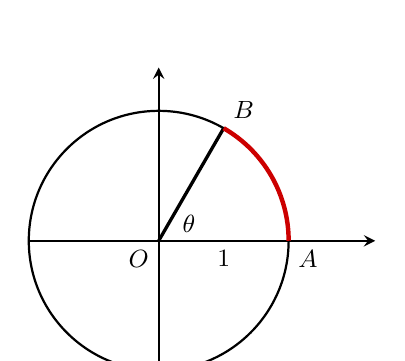
\begin{tikzpicture}[>=stealth, scale=1.1, font=\small]
  \draw[->, thick] (-1.5, 0) -- (2.5, 0);
  \draw[->, thick] (0, -1.5) -- (0, 2);
  \draw[thick] (0, 0) circle (1.5cm);
  \coordinate (O) at (0, 0);
  \coordinate (A) at (1.5, 0);
  \coordinate (B) at (60:1.5);
  \draw[very thick] (O) -- (B);
  \draw[ultra thick, red!80!black] (A) arc (0:60:1.5);
  \node[below left] at (O) {$O$};
  \node[below right] at (A) {$A$};
  \node[above right] at (B) {$B$};
  \node at (0.35, 0.2) {$\theta$};
  \node[below] at (0.75, 0) {$1$};
\end{tikzpicture}
\caption{單位圓弧長度量角}
\label{fig:b3-fig2-13-1}
\end{minipage}
\end{figure}

單位圓半圓周長是一個無理數，約 $3.14159\dots\dots$，四捨五入後略為 $3.1416$ 通常以符號 $\pi$ 記之；即 $\pi = \text{單位圓半圓周長} = 3.14159\dots\dots \doteq 3.1416$.

考慮兩圓，半徑分別為 1 與 $r$. 考慮它們夾在一個角 $\angle\theta$ 內部的圓弧 $\wideparen{AB}$ 與 $\wideparen{A'B'}$，若用弧度制，則 $\wideparen{AB}$ 弧長 $= \theta$，今欲證

\begin{proposition}
以 $r$ 為半徑，對圓心張出圓心角 $\angle\theta$ 的圓弧，弧長為 $r\theta$，亦即
\[ \wideparen{A'B'} \text{ 弧長} = r\theta \]
\end{proposition}

\begin{figure}[H]
\centering
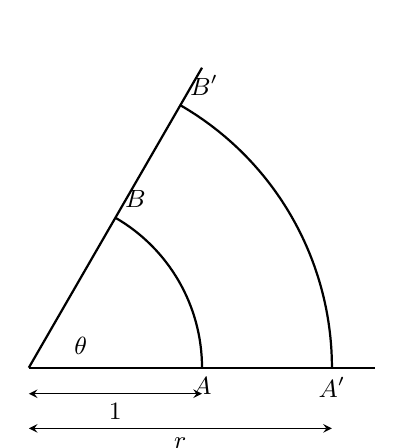
\begin{tikzpicture}[>=stealth, scale=1.1, font=\small]
  \coordinate (O) at (0, 0);
  \draw[thick] (O) -- (4, 0);
  \draw[thick] (O) -- (60:4);
  \draw[thick] (2, 0) arc (0:60:2);
  \draw[thick] (3.5, 0) arc (0:60:3.5);
  \node[below] at (2, 0) {$A$};
  \node[above right] at (60:2) {$B$};
  \node[below] at (3.5, 0) {$A'$};
  \node[above right] at (60:3.5) {$B'$};
  \node at (0.6, 0.25) {$\theta$};
  \draw[<->] (0, -0.3) -- (2, -0.3) node[midway, below] {$1$};
  \draw[<->] (0, -0.7) -- (3.5, -0.7) node[midway, below] {$r$};
\end{tikzpicture}
\caption{同心圓弧長與半徑成正比}
\label{fig:b3-fig2-14}
\end{figure}

\begin{proof}
弧長 $\wideparen{AB}$ 與 $\wideparen{A'B'}$ 其實分別是折線 $AC_1 \cup C_1 C_2 \cup \dots \cup C_n B$ 與 $A'C_1' \cup C_1' C_2' \cup \dots \cup C_n' B'$ 當分割 $C_1, C_2, \dots, C_n$ 為無限細密時的極限（見圖 2-15）.

但因 $\overline{OA'} = r\overline{OA}$, $\overline{OC_1'} = r\overline{OC_1}$，得 $\triangle AOC_1 \sim \triangle A'OC_1'$，故 $\overline{A'C_1'} = r\overline{AC_1}$.

同理 $\overline{C_1' C_2'} = r\overline{C_1 C_2}, \dots, \overline{C_n' B'} = r\overline{C_n B}$.

故沿 $\wideparen{A'B'}$ 之折線長
\[ \overline{A'C_1'} + \overline{C_1'C_2'} + \dots + \overline{C_n'B'} \]
為沿 $\wideparen{AB}$ 之折線長
\[ \overline{AC_1} + \overline{C_1 C_2} + \dots + \overline{C_n B} \]
之 $r$ 倍. 取分割為無限細密時之極限，得 $\wideparen{A'B'}$ 弧長為 $\wideparen{AB}$ 弧長之 $r$ 倍，亦即
\[ \wideparen{A'B'} \text{ 弧長} = r\wideparen{AB} \text{ 弧長} = r\theta \qedhere \]
\end{proof}

\begin{figure}[H]
\centering
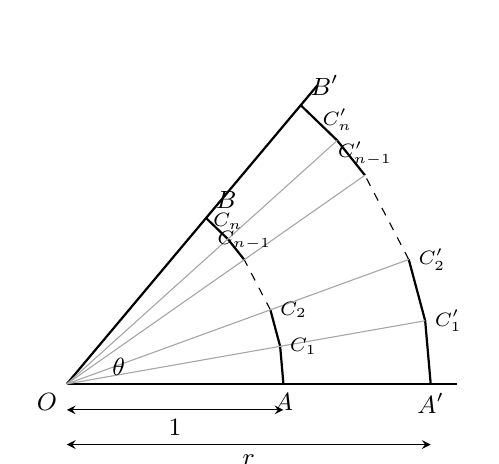
\begin{tikzpicture}[>=stealth, scale=1.1, font=\small]
  \coordinate (O) at (0, 0);
  \draw[thick] (O) -- (4.5, 0);
  \draw[thick] (O) -- (50:4.5);

  % Inner arc & points
  \coordinate (A) at (2.5, 0);
  \coordinate (c1) at (10:2.5);
  \coordinate (c2) at (20:2.5);
  \coordinate (cnm1) at (35:2.5);
  \coordinate (cn) at (42:2.5);
  \coordinate (B) at (50:2.5);
  \draw[thick] (A) -- (c1) -- (c2);
  \draw[dashed] (c2) -- (cnm1);
  \draw[thick] (cnm1) -- (cn) -- (B);

  % Outer arc & points
  \coordinate (Aprime) at (4.2, 0);
  \coordinate (c1p) at (10:4.2);
  \coordinate (c2p) at (20:4.2);
  \coordinate (cnm1p) at (35:4.2);
  \coordinate (cnp) at (42:4.2);
  \coordinate (Bprime) at (50:4.2);
  \draw[thick] (Aprime) -- (c1p) -- (c2p);
  \draw[dashed] (c2p) -- (cnm1p);
  \draw[thick] (cnm1p) -- (cnp) -- (Bprime);

  % Radial lines
  \draw[gray!70] (O) -- (c1p);
  \draw[gray!70] (O) -- (c2p);
  \draw[gray!70] (O) -- (cnm1p);
  \draw[gray!70] (O) -- (cnp);

  % Labels
  \node[below] at (A) {$A$};
  \node[below] at (Aprime) {$A'$};
  \node[above right] at (B) {$B$};
  \node[above right] at (Bprime) {$B'$};
  \node[right] at (c1) {\scriptsize $C_1$};
  \node[right] at (c1p) {\scriptsize $C_1'$};
  \node[right] at (c2) {\scriptsize $C_2$};
  \node[right] at (c2p) {\scriptsize $C_2'$};
  \node[above] at (cnm1) {\scriptsize $C_{n-1}$};
  \node[above] at (cnm1p) {\scriptsize $C_{n-1}'$};
  \node[above] at (cn) {\scriptsize $C_n$};
  \node[above] at (cnp) {\scriptsize $C_n'$};
  \node[below left] at (O) {$O$};
  \node at (0.6, 0.2) {$\theta$};

  \draw[<->] (0, -0.3) -- (2.5, -0.3) node[midway, below] {$1$};
  \draw[<->] (0, -0.7) -- (4.2, -0.7) node[midway, below] {$r$};
\end{tikzpicture}
\caption{極限分割與弧長比例}
\label{fig:b3-fig2-15}
\end{figure}

這個命題舉出弧度制的一個好處. 以下我們都採用弧度制，必要用 360 度制時會特別聲明.

一周角便是射線正向旋轉一整圈又回到原來位置的角. 因單位圓圓周長為 $2\pi$，故周角的角度亦為 $2\pi$.

\begin{corollary}
一個以 $r$ 為半徑的圓，其圓周長為 $2\pi r$.
\end{corollary}

\begin{proof}
當上述命題中之角度 $\theta$ 取為周角 $2\pi$，即得圓周長為 $2\pi r$.
\end{proof}

\textbf{注意}：半周角所對單位圓弧長為單位圓半周長 $\pi$，故為 $\pi$ 弧度，直角所夾的單位圓圓弧長 $\frac{\pi}{2}$，故其在弧度制下之度量為 $\frac{\pi}{2}$ 弧度.

\subsubsection*{作業 1}
採用弧度制，下列角度若干？
\begin{enumerate}[label=\roman*), leftmargin=2.5em]
  \item $\frac{1}{16}$ 周角 \qquad\qquad ii) $\frac{1}{3}$ 周角
  \item[iii)] $\frac{1}{6}$ 周角 \qquad\qquad iv) $\frac{1}{10}$ 周角
\end{enumerate}

\begin{example}
弧度制與 360 度制都是數量化角的度量制度\footnote{此二制的換算表見附錄二表 3.}，其間換算關係可如下求得：

因一半圓所對的圓心角為一平角. 等於 $180^\circ$，故有
\[ 180^\circ = \pi \text{ 弧度} \]
所以
\[ 1^\circ = \frac{\pi}{180} \text{ 弧度} \doteq 0.0175 \text{ 弧度} \]
\[ 1 \text{ 弧度} = \left(\frac{180}{\pi}\right)^\circ \doteq (57.296)^\circ = 57^\circ 17' 45'' \qedhere \]
\end{example}

\subsubsection*{作業 2}
給了 360 度制下的角度，試求其弧度
\begin{enumerate}[label=\roman*), leftmargin=2.5em]
  \item $50^\circ$ \qquad\qquad ii) $42^\circ 24' 35''$ \qquad\qquad iii) $135^\circ$ \qquad\qquad iv) $210^\circ$
\end{enumerate}

\subsubsection*{作業 3}
試求下列角度在 360 度制下之度數
\begin{enumerate}[label=\roman*), leftmargin=2.5em]
  \item $\frac{3\pi}{4}$ \qquad\qquad ii) $2$ \qquad\qquad iii) $\frac{\pi}{6}$ \qquad\qquad iv) $\frac{7}{5}$
\end{enumerate}

\subsubsection*{庚、扇形}

既然我們已經提過用折線逼近圓弧，不妨接下去考慮扇形面積及圓面積：

所謂扇形是一個在圓內夾在自圓心出發的兩根射線間的部分，其頂角則為這兩射線所夾的角度，這角度可以是 0 到 $2\pi$ 間的任何角度. 如下圖 (2-16) 之扇形常記以 $\sphericalangle OAB$ 或直接寫成 扇形 $OAB$. $OA$ 或 $OB$ 之長稱為扇形之徑，即 $\overline{OA}$ 或 $\overline{OB}$.

\begin{figure}[H]
\centering
\begin{minipage}{0.48\textwidth}
\centering
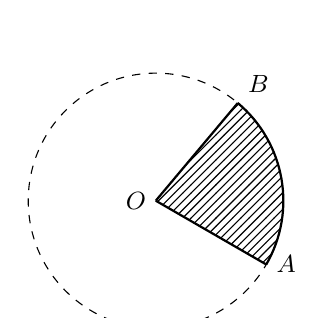
\begin{tikzpicture}[>=stealth, scale=0.9, font=\small]
  \coordinate (O) at (0, 0);
  \draw[dashed] (O) circle (1.8cm);
  \coordinate (A) at (-30:1.8);
  \coordinate (B) at (50:1.8);
  \draw[thick] (O) -- (A) node[right] {$A$};
  \draw[thick] (O) -- (B) node[above right] {$B$};
  \draw[thick] (A) arc (-30:50:1.8);
  \fill[pattern=north east lines] (O) -- (A) arc (-30:50:1.8) -- cycle;
  \node[left] at (O) {$O$};
\end{tikzpicture}
\end{minipage}
\hfill
\begin{minipage}{0.48\textwidth}
\centering
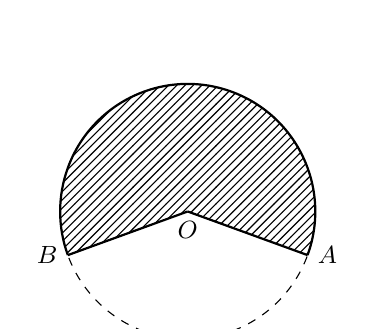
\begin{tikzpicture}[>=stealth, scale=0.9, font=\small]
  \coordinate (O) at (0, 0);
  \draw[dashed] (O) circle (1.8cm);
  \coordinate (A) at (-20:1.8);
  \coordinate (B) at (200:1.8);
  \draw[thick] (O) -- (A) node[right] {$A$};
  \draw[thick] (O) -- (B) node[left] {$B$};
  \draw[thick] (A) arc (-20:200:1.8);
  \fill[pattern=north east lines] (O) -- (A) arc (-20:200:1.8) -- cycle;
  \node[below] at (O) {$O$};
\end{tikzpicture}
\end{minipage}
\caption{扇形之頂角範圍}
\label{fig:b3-fig2-16}
\end{figure}

\begin{proposition}[扇形面積]
若扇形 $OAB$ 之頂角為 $\theta$，半徑為 $r$，則其面積為 $\frac{1}{2}r^2\theta$.
\end{proposition}

\begin{proof}
設折線 $AC_1 \cup C_1 C_2 \cup \dots \cup C_n B$ 如圖 2-17 逼近 $\wideparen{AB}$，則
\[ \triangle OAC_1,\; \triangle OC_1 C_2,\; \dots,\; \triangle OC_n B \]
面積的和亦逼近扇形 $AOB$ 的面積.

但這些小三角形之高很逼近於 $r$，設其頂角分別為 $\theta_1, \theta_2, \dots, \theta_{n+1}$，則 $\theta = \theta_1 + \theta_2 + \dots + \theta_{n+1}$ 而小三角形底邊長則分別逼近於弧長 $\wideparen{AC_1}, \wideparen{C_1 C_2}, \dots, \wideparen{C_n B}$. 亦即分別逼近於 $r\theta_1, r\theta_2, \dots, r\theta_{n+1}$.

故小三角形之面積和逼近於
\[ \frac{1}{2}r(r\theta_1) + \frac{1}{2}r(r\theta_2) + \dots + \frac{1}{2}r(r\theta_{n+1}) = \frac{1}{2}r^2\theta \]
故取了無限細密的分割之極限後，得
\[ \text{扇形 } OAB \text{ 面積} = \frac{1}{2}r^2\theta \qedhere \]
\end{proof}

\begin{figure}[H]
\centering
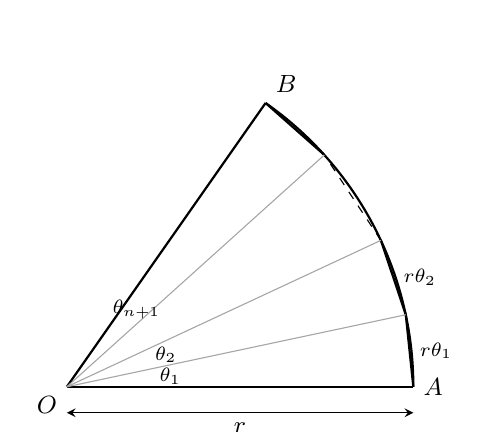
\begin{tikzpicture}[>=stealth, scale=1.1, font=\small]
  \coordinate (O) at (0, 0);
  \draw[thick] (O) -- (4, 0) node[right] {$A$};
  \draw[thick] (O) -- (55:4) node[above right] {$B$};
  \draw[thick] (4, 0) arc (0:55:4);

  % Subdivisions
  \coordinate (c1) at (12:4);
  \coordinate (c2) at (25:4);
  \coordinate (cn) at (42:4);

  \draw[thick] (4, 0) -- (c1) node[midway, right] {\scriptsize $r\theta_1$};
  \draw[thick] (c1) -- (c2) node[midway, right] {\scriptsize $r\theta_2$};
  \draw[dashed] (c2) -- (cn);
  \draw[thick] (cn) -- (55:4);

  \draw[gray!70] (O) -- (c1);
  \draw[gray!70] (O) -- (c2);
  \draw[gray!70] (O) -- (cn);

  \node at (6:1.2) {\scriptsize $\theta_1$};
  \node at (18:1.2) {\scriptsize $\theta_2$};
  \node at (48:1.2) {\scriptsize $\theta_{n+1}$};
  \node[below left] at (O) {$O$};
  \draw[<->] (0, -0.3) -- (4, -0.3) node[midway, below] {$r$};
\end{tikzpicture}
\caption{扇形面積極限逼近}
\label{fig:b3-fig2-17}
\end{figure}

\begin{corollary}[圓面積]
圓面積為 $\pi r^2$.
\end{corollary}

\begin{proof}
若取頂角 $\theta$ 為周角 $2\pi$ 時，扇形變成圓本身，故圓面積為
\[ \frac{1}{2}r^2\theta = \frac{1}{2}r^2(2\pi) = \pi r^2 \qedhere \]
\end{proof}

\subsection*{習題 2-1}

\begin{enumerate}[label=\arabic*., leftmargin=2em]
  \item 設圓的半徑為 2，試求下列各圓心角所對之弧長.
  \begin{enumerate}[label=(\roman*), leftmargin=2.5em]
    \item $30^\circ$ \qquad (ii) $45^\circ$ \qquad (iii) $60^\circ$ \qquad (iv) $120^\circ$
    \item[(v)] $150^\circ$ \qquad (vi) $225^\circ$ \qquad (vii) $270^\circ$
  \end{enumerate}
  \item 試求上題中各圓心角所張扇形之面積.
  \item 設腳踏車輪的直徑為 70 公分，試求旋轉 500 圈所行之距離.
  \begin{flushright}
  \begin{tikzpicture}[>=stealth, scale=0.85, baseline=(current bounding box.center)]
    \draw[thick] (0, 0) circle (1.5cm);
    \fill (0, 0) circle (2pt) node[left] {太陽};
    \coordinate (E1) at (60:1.5);
    \coordinate (E2) at (85:1.5);
    \draw (0, 0) -- (E1);
    \draw (0, 0) -- (E2);
    \fill[pattern=north east lines] (0, 0) -- (E1) arc (60:85:1.5) -- cycle;
    \fill (E1) circle (2pt) node[right] {地球};
  \end{tikzpicture}
  \end{flushright}
  \item 某甲騎着自行車走了一哩路，車輪直徑為 28 吋，試問車輪轉了幾圈？所轉周角的角度若干？（註：1 哩 = 5280 呎）
  \item 時鐘從八點十分到九點，時針、分針、秒針經過的角度各若干？
  \item 設一正方形之邊長為 $a$，用相鄰二邊為直徑向內各作一圓，求這兩個圓共同部分的面積.
  \item 假設太陽系中的行星以太陽為中心做等速圓周運動，（事實上是以太陽為焦點之橢圓為行進軌道的）地球一年（算它 365 天，或 12 個月）繞一周. 太陽與地球的距離已知為 $1.455 \times 10^8$ 公里. 試問地球走了一個月或一星期（七天）所相應的轉過的圓心角為若干，所對應的掃過的扇形面積若干？（如圖 2-18）
  \item 
  \begin{enumerate}[label=(\roman*), leftmargin=2.5em]
    \item 將一四邊形分割成兩個三角形，證明四邊形內角和為 $2\pi$. 一般地將一個 $n$ 邊形分割成 $(n-2)$ 個三角形，證明 $n$ 邊形內角和為 $(n-2)\pi$.
    \item 考慮一質點沿一個 $n$ 邊形（不拘凹凸）的邊逆時針運動檢驗它方向的變化情形，舉例說明這質點繞一圈回到原來位置時方向正好轉了 $2\pi$. 據此再證明 $n$ 邊形的內角和為 $(n-2)\pi$.
  \end{enumerate}
\end{enumerate}

\subsection{三角函數的定義}
\label{subsec:b3-2-2}

國中已講過銳角的三角函數，在那裏我們記得三角函數其實不過是直角三角形各邊的比例. 例如正弦、餘弦只是直角邊與斜邊之比，正切、餘切則為兩直角邊之比.

如果將這直角三角形各邊比例預先根據一個內角的大小相當準確地列出一張表，稱為\textbf{三角函數表}，便可拿出去航海，這是十八世紀所謂「書本航海」的開始. 在航海史上是個新的紀元.

它的基本精神在於利用相似三角形的原理. 只要知道原來地理或天文上圖形的一邊，便可把它縮成紙上作業，利用基本的直觀幾何的原理並參照編好的三角函數表來求得地理或天文圖形上未知的邊長. 這樣的過程在國中的三角測量裏，我們已經提及，而在本章第 5 節中，我們將要作進一步的討論.

其實三角函數的好處，不止在於三角測量. 自然界的各種波動竟是正弦函數（或餘弦函數）. 這現象在電磁學的發展上，一直佔著很重要的地位. 這些會在下節的例題中提及.

\subsubsection*{甲、銳角的三角函數}

先複習一下國中提過的，銳角三角函數的定義.

給了一個銳角 $\angle(\theta; \mathbf{r}_1, \mathbf{r}_2)$，銳角意為 $0 < \theta < \frac{\pi}{2}$，設 $A$ 為 $\mathbf{r}_1$ 與 $\mathbf{r}_2$ 的公共起點，在 $\mathbf{r}_1$ 邊上取一點 $C$，在 $C$ 上做 $\mathbf{r}_1$ 的垂線交 $\mathbf{r}_2$ 於 $B$，畫 $\triangle ABC$，如圖 2-19.

\begin{figure}[H]
\centering
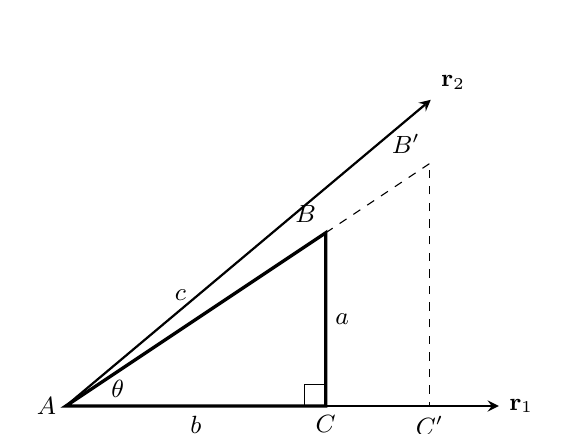
\begin{tikzpicture}[>=stealth, scale=1.1, font=\small]
  \coordinate (A) at (0, 0);
  \coordinate (C) at (3, 0);
  \coordinate (B) at (3, 2);
  \coordinate (Cprime) at (4.2, 0);
  \coordinate (Bprime) at (4.2, 2.8);

  \draw[->, thick] (A) -- (5, 0) node[right] {$\mathbf{r}_1$};
  \draw[->, thick] (A) -- (40:5.5) node[above right] {$\mathbf{r}_2$};

  \draw[very thick] (A) -- (C) -- (B) -- cycle;
  \draw (C) rectangle ++(-0.25, 0.25);

  \draw[dashed] (B) -- (Bprime);
  \draw[dashed] (C) -- (Cprime) -- (Bprime);

  \node[left] at (A) {$A$};
  \node[below] at (C) {$C$};
  \node[above left] at (B) {$B$};
  \node[below] at (Cprime) {$C'$};
  \node[above left] at (Bprime) {$B'$};

  \node at (0.6, 0.2) {$\theta$};
  \node[below] at (1.5, 0) {$b$};
  \node[right] at (3, 1) {$a$};
  \node[above left] at (1.5, 1.1) {$c$};
\end{tikzpicture}
\caption{直角三角形與銳角三角函數}
\label{fig:b3-fig2-19}
\end{figure}

設 $\overline{AB} = c$, $\overline{AC} = b$, $\overline{BC} = a$.

則張角 $\angle\theta$ 的六個三角函數值是用直角 $\triangle ABC$ 各邊的兩兩比例來定義的，我們稱 $BC$ 為 $\angle A$ 的對邊，$AC$ 為 $\angle A$ 的鄰邊，$AB$ 為斜邊，它們的長按序記為 $a, b, c$，則規定
\begin{align*}
\sin\theta &= \angle A\text{ 的正弦} = \frac{\text{對邊}}{\text{斜邊}} = \frac{a}{c} \\
\cos\theta &= \angle A\text{ 的餘弦} = \frac{\text{鄰邊}}{\text{斜邊}} = \frac{b}{c} \\
\tan\theta &= \angle A\text{ 的正切} = \frac{\text{對邊}}{\text{鄰邊}} = \frac{a}{b} \\
\cot\theta &= \angle A\text{ 的餘切} = \frac{\text{鄰邊}}{\text{對邊}} = \frac{b}{a} \\
\sec\theta &= \angle A\text{ 的正割} = \frac{\text{斜邊}}{\text{鄰邊}} = \frac{c}{b} \\
\csc\theta &= \angle A\text{ 的餘割} = \frac{\text{斜邊}}{\text{對邊}} = \frac{c}{a}
\end{align*}

雖然以上的定義是依據特定的 $\triangle ABC$ 做出的，要注意的是，所取的邊的比值與所取的直角三角形無關. 理由是：$C$ 是 $\mathbf{r}_1$ 上任取的點，取定後，以之為垂足所做的直角三角形均相似，因此邊的比值總是相等的. 而另一方面，若不在 $\mathbf{r}_1$ 上取點而改在 $\mathbf{r}_2$ 上取點 $B'$，並以之為垂足做 $\triangle AB'C'$，則由圖易知以 $\triangle AB'C'$ 的邊的比值來定義三角函數結果是相同的，此時 $\overline{B'C'}$ 為 $\angle A$ 的對邊，$\overline{AB'}$ 為 $\angle A$ 的鄰邊，$\overline{AC'}$ 為斜邊.

由以上討論可知：給了一個銳角 $\angle\theta$，所對應的六個數值（比值）只與其角度 $\theta$ 有關，$\theta$ 變時，數值隨之而變，此六數值為相應於 $\theta$ 的應變量，故為 $\theta$ 的函數. 又因其函數值與三角形有關，故稱為\textbf{三角函數}，依次記為：
\begin{align*}
\sin\theta &= \theta\text{ 的正弦函數} \\
\cos\theta &= \theta\text{ 的餘弦函數} \\
\tan\theta &= \theta\text{ 的正切函數} \\
\cot\theta &= \theta\text{ 的餘切函數} \\
\sec\theta &= \theta\text{ 的正割函數} \\
\csc\theta &= \theta\text{ 的餘割函數}
\end{align*}

\begin{example}
試比較 $\sin 55^\circ$ 與 $\cos 55^\circ$ 的大小.
\end{example}

\begin{proof}[解]
做 $\triangle ABC$ 使 $\angle A = 55^\circ$, $\angle B = \text{直角}$，則 $\angle C = 90^\circ - 55^\circ = 35^\circ$，而 $\angle A > \angle C$.

三角形內大角對大邊，故有 $\overline{AB} < \overline{BC}$，所以
\[ \sin 55^\circ = \frac{\overline{BC}}{\overline{AC}} > \frac{\overline{AB}}{\overline{AC}} = \cos 55^\circ \qedhere \]
\end{proof}

\begin{figure}[H]
\centering
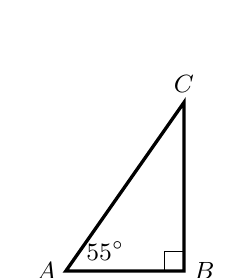
\begin{tikzpicture}[>=stealth, scale=1.0, font=\small]
  \coordinate (A) at (0, 0);
  \coordinate (B) at (1.5, 0);
  \coordinate (C) at (1.5, 2.14);
  \draw[very thick] (A) -- (B) -- (C) -- cycle;
  \draw (B) rectangle ++(-0.25, 0.25);
  \node[left] at (A) {$A$};
  \node[right] at (B) {$B$};
  \node[above] at (C) {$C$};
  \node at (0.5, 0.25) {$55^\circ$};
\end{tikzpicture}
\caption{$\triangle ABC$ 之角邊關係}
\label{fig:b3-fig2-20}
\end{figure}

\subsubsection*{作業 4}
試比較下列各組函數值之大小.
\begin{enumerate}[label=\roman*), leftmargin=2.5em]
  \item $\sin 40^\circ,\; \cos 40^\circ$ \qquad ii) $\tan 15^\circ,\; \cot 15^\circ$ \qquad iii) $\sec 55^\circ,\; \csc 55^\circ$
\end{enumerate}

\textbf{注意}\quad 到目前為止，三角函數的定義域（即自變數變化的範圍）為 $0 < \theta < \frac{\pi}{2}$.

\begin{example}
試求銳角 $\frac{\pi}{4}$ 之正弦、餘弦與正切.
\end{example}

\begin{proof}[解]
繪 $\triangle ABC$ 使得 $\angle A = \frac{\pi}{4}$，$\angle C = \text{直角}$，則 $\triangle ABC$ 為等腰，$\overline{AC} = \overline{BC}$.

由畢氏定理 $\overline{AC}^2 + \overline{BC}^2 = \overline{AB}^2$，得 $\overline{AB} = \sqrt{2}\;\overline{AC}$.

所以
\begin{align*}
\sin\frac{\pi}{4} &= \sin A = \frac{\overline{BC}}{\overline{AB}} = \frac{1}{\sqrt{2}} \\
\cos\frac{\pi}{4} &= \cos A = \frac{\overline{AC}}{\overline{AB}} = \frac{1}{\sqrt{2}} \\
\tan\frac{\pi}{4} &= \tan A = \frac{\overline{BC}}{\overline{AC}} = 1 \qedhere
\end{align*}
\end{proof}

\begin{figure}[H]
\centering
\begin{minipage}{0.48\textwidth}
\centering
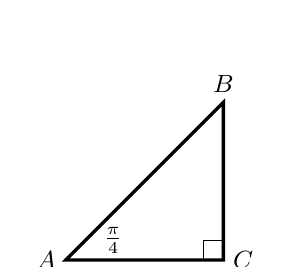
\begin{tikzpicture}[>=stealth, scale=1.0, font=\small]
  \coordinate (A) at (0, 0);
  \coordinate (C) at (2, 0);
  \coordinate (B) at (2, 2);
  \draw[very thick] (A) -- (C) -- (B) -- cycle;
  \draw (C) rectangle ++(-0.25, 0.25);
  \node[left] at (A) {$A$};
  \node[right] at (C) {$C$};
  \node[above] at (B) {$B$};
  \node at (0.6, 0.25) {$\frac{\pi}{4}$};
\end{tikzpicture}
\caption{等腰直角三角形}
\label{fig:b3-fig2-21}
\end{minipage}
\hfill
\begin{minipage}{0.48\textwidth}
\centering
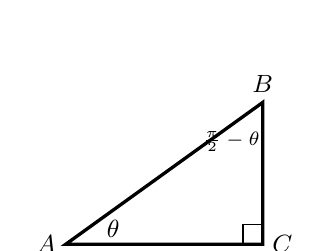
\begin{tikzpicture}[>=stealth, scale=1.0, font=\small]
  \coordinate (A) at (0, 0);
  \coordinate (C) at (2.5, 0);
  \coordinate (B) at (2.5, 1.8);
  \draw[very thick] (A) -- (C) -- (B) -- cycle;
  \draw (C) rectangle ++(-0.25, 0.25);
  \node[left] at (A) {$A$};
  \node[right] at (C) {$C$};
  \node[above] at (B) {$B$};
  \node at (0.6, 0.2) {$\theta$};
  \node at (2.1, 1.3) {\scriptsize $\frac{\pi}{2}-\theta$};
\end{tikzpicture}
\caption{餘角幾何關係}
\label{fig:b3-fig2-22}
\end{minipage}
\end{figure}

\subsubsection*{作業 5}
試求銳角 $\frac{\pi}{3}$ 與 $\frac{\pi}{6}$ 之三角函數，然後將 $\frac{\pi}{6}, \frac{\pi}{4}, \frac{\pi}{3}$ 各角的三角函數值列表整理.

一個銳角的角度若為 $\theta$，則其餘角為 $\frac{\pi}{2}-\theta$，由銳角三角函數的定義，及圖 2-21 可得：
\begin{align*}
\sin\left(\frac{\pi}{2}-\theta\right) &= \frac{\overline{AC}}{\overline{AB}} = \cos\theta \\
\cos\left(\frac{\pi}{2}-\theta\right) &= \frac{\overline{BC}}{\overline{AB}} = \sin\theta \\
\tan\left(\frac{\pi}{2}-\theta\right) &= \frac{\overline{AC}}{\overline{BC}} = \cot\theta
\end{align*}

此即：一個銳角之餘角的正弦即為此銳角之餘弦，而其餘角之餘弦為此角的正弦. 同樣的關係也存在於正切與餘切，正割與餘割之間. 總結上述，我們有

\begin{proposition}[銳角的餘角公式]
\begin{align*}
\sin\left(\frac{\pi}{2}-\theta\right) &= \cos\theta,\quad \tan\left(\frac{\pi}{2}-\theta\right) = \cot\theta \\
\sec\left(\frac{\pi}{2}-\theta\right) &= \csc\theta
\end{align*}
\end{proposition}

\begin{example}
設 $\theta_1 < \theta_2$ 為二銳角，試分別比較此二銳角之正弦與餘弦.
\end{example}

\begin{proof}[解]
以 $\mathbf{r}_1$ 為始邊做張角 $\theta_1$ 與 $\theta_2$ 各有終邊 $\mathbf{r}_2, \mathbf{r}_3$. 設頂點為 $A$. 在 $\mathbf{r}_1$ 上取一點 $B$，在 $B$ 上做 $\mathbf{r}_1$ 垂線各交 $\mathbf{r}_2, \mathbf{r}_3$ 於 $C, D$. 則因 $\angle ACB$ 亦為銳角，$\angle ACD$ 必為鈍角，而一三角形內最多只有一個鈍角，故在 $\triangle ACD$ 中，$\angle ACD > \angle ADC$. 因三角形內大角對大邊故有 $\overline{AD} > \overline{AC}$.

今
\[ \cos\theta_1 = \frac{\overline{AB}}{\overline{AC}},\qquad \cos\theta_2 = \frac{\overline{AB}}{\overline{AD}} \]
故有 $\cos\theta_1 > \cos\theta_2$.

同理 $\cos\left(\frac{\pi}{2}-\theta_1\right) < \cos\left(\frac{\pi}{2}-\theta_2\right)$.

又由命題 3 知 $\sin\theta_1 = \cos\left(\frac{\pi}{2}-\theta_1\right)$，$\sin\theta_2 = \cos\left(\frac{\pi}{2}-\theta_2\right)$，故有 $\sin\theta_1 < \sin\theta_2$.
\end{proof}

\begin{figure}[H]
\centering
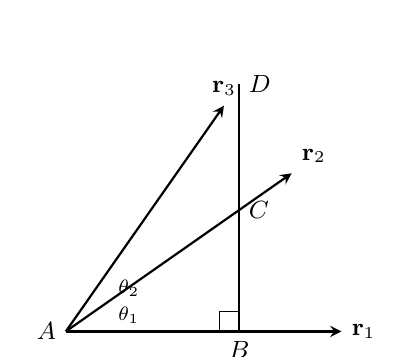
\begin{tikzpicture}[>=stealth, scale=1.0, font=\small]
  \coordinate (A) at (0, 0);
  \draw[->, thick] (A) -- (3.5, 0) node[right] {$\mathbf{r}_1$};
  \draw[->, thick] (A) -- (35:3.5) node[above right] {$\mathbf{r}_2$};
  \draw[->, thick] (A) -- (55:3.5) node[above] {$\mathbf{r}_3$};

  \coordinate (B) at (2.2, 0);
  \coordinate (C) at (2.2, 1.54);
  \coordinate (D) at (2.2, 3.14);

  \draw[thick] (B) -- (D);
  \draw (B) rectangle ++(-0.25, 0.25);

  \node[left] at (A) {$A$};
  \node[below] at (B) {$B$};
  \node[right] at (C) {$C$};
  \node[right] at (D) {$D$};

  \node at (0.8, 0.2) {\scriptsize $\theta_1$};
  \node at (0.8, 0.55) {\scriptsize $\theta_2$};
\end{tikzpicture}
\caption{銳角單調性幾何證明}
\label{fig:b3-fig2-23}
\end{figure}

\subsubsection*{作業 6}
\begin{enumerate}[label=\roman*), leftmargin=2.5em]
  \item 試比較銳角 $\frac{\pi}{6}, \frac{\pi}{4}, \frac{\pi}{3}$ 之正弦、餘弦與正切.
  \item 試說明在定義域 $0 < \theta < \frac{\pi}{2}$ 內，$\sin\theta$ 與 $\tan\theta$ 為增函數，$\cos\theta$ 為減函數.
\end{enumerate}

由定義，我們可直接得到以下關係式

\begin{proposition}
\begin{align*}
\sin\theta \cdot \csc\theta &= 1 \\
\cos\theta \cdot \sec\theta &= 1 \\
\tan\theta \cdot \cot\theta &= 1
\end{align*}
（即同一角度的正弦與餘割，餘弦與正割，正切與餘切互為倒數）
及
\[ \tan\theta = \frac{\sin\theta}{\cos\theta},\qquad \cot\theta = \frac{\cos\theta}{\sin\theta} \]
\end{proposition}

三角函數表是把 0 度到 45 度的銳角（每 $10'$ 一計，並標出相應的弧度）的三角函數值利用直角三角形邊與邊的比算出，以小數表示橫列出來，所做成的表（附錄），有了這表，便可反過來再利用相似三角形原理計算出：給了一已知邊及已知角的直角三角形的其他邊長. 計算時就只要在表中把所需之已知角的某些函數值查出，代入關係式即可. 在航海上，天文上，地形測量上都很便利，今只以國中已學過的力的分解來看.

\begin{example}
有一重 $m$ 克的物體放在一坡度 $36^\circ$ 的斜面上，試問此斜面受力多少？
\end{example}

\begin{proof}[解]
物體向地心的重力為 $mg$，$g$ 為重力加速度. 此力分解為兩個互相垂直的力：向斜面的壓力 $\vec{OA}$ 及沿斜面下滑的力 $\vec{OB}$. 斜面所受壓力與重力 $mg$ 成 $36^\circ$ 角，設此壓力為 $P$ 則
\[ \frac{P}{mg} = \cos 36^\circ \]
\begin{figure}[H]
\centering
\begin{tikzpicture}[>=stealth, scale=1.0, font=\small]
  % Inclined plane 36 degrees
  \coordinate (O_ground) at (0, 0);
  \draw[thick] (O_ground) -- (4, 0);
  \draw[thick] (O_ground) -- (36:4);
  \node at (0.8, 0.25) {$36^\circ$};

  % Object on incline
  \coordinate (M) at (36:2.5);
  \begin{scope}[rotate around={36:(M)}]
    \draw[thick, fill=gray!20] ($(M)+(-0.4, 0)$) rectangle ($(M)+(0.4, 0.5)$);
    \coordinate (Center) at ($(M)+(0, 0.25)$);
  \end{scope}

  % Forces from Center
  \draw[->, very thick] (Center) -- ++(0, -1.8) node[below] {$mg$};
  \draw[->, very thick] (Center) -- ++(-54:1.45) node[below right] {$A$} node[midway, right] {$P = {?}$};
  \draw[->, very thick] (Center) -- ++(216:1.05) node[left] {$B$};
  \draw[dashed] ($(Center)+(0, -1.8)$) -- ($(Center)+(-54:1.45)$);
  \draw[dashed] ($(Center)+(0, -1.8)$) -- ($(Center)+(216:1.05)$);

  \fill (Center) circle (1.5pt) node[above right] {$O$};
\end{tikzpicture}
\caption{斜面重力正交分解}
\label{fig:b3-fig2-24}
\end{figure}
查三角函數表知 $\cos 36^\circ = 0.8090$，
\[ \therefore\quad P = mg \cdot \cos 36^\circ = 0.809 mg\text{ 克} \qedhere \]
\end{proof}

\subsubsection*{作業 7}
\begin{enumerate}[label=\roman*), leftmargin=2.5em]
  \item 設有一梯子靠牆放與牆成 $15^\circ$ 角，梯長 6 公尺，問梯頂到牆角距離.
  \item 設一等邊三角形之邊長為 5，試求其高.
  \item 求正六邊形中心到其邊所做垂線之長.
\end{enumerate}

\subsubsection*{乙、三角函數}

現在我們要定義廣義的三角函數.

由於實際的需要，我們把三角函數定義在實數上來代替在角上的定義，以下談到角度我們都固定採用弧度制.

取平面一座標系 $(O; X, Y)$，使 $\vec{OX}$ 到 $\vec{OY}$ 的轉角為 $+\frac{\pi}{2}$（必要時，這樣的座標系稱為正向座標系）.

\begin{definition}
對任一實數 $t$，考慮一廣義有向角 $\angle(\theta; \mathbf{r}_1, \mathbf{r}_2)$，使其始邊 $\mathbf{r}_1 = \vec{OX}$ 且 $\angle\theta$ 的角度 $\theta$ 等於 $t$. 在終邊上取一點 $P(x, y)$，使得 $\overline{OP} = 1$. 當下列各式右端有意義時（即分母不為 0 時）定義各三角函數如下：
\begin{align*}
\text{正弦}\quad \sin t &= \frac{y}{1} = y \\
\text{餘弦}\quad \cos t &= \frac{x}{1} = x \\
\text{正切}\quad \tan t &= \frac{y}{x} \\
\text{餘切}\quad \cot t &= \frac{x}{y} \\
\text{正割}\quad \sec t &= \frac{1}{x} \\
\text{餘割}\quad \csc t &= \frac{1}{y}
\end{align*}
\end{definition}

\begin{figure}[H]
\centering
\begin{tikzpicture}[>=stealth, scale=1.1, font=\small]
  \draw[->, thick] (-1.5, 0) -- (2.2, 0) node[right] {$X$};
  \draw[->, thick] (0, -1.5) -- (0, 2) node[above] {$Y$};
  \draw[thick] (0, 0) circle (1.5cm);

  \coordinate (O) at (0, 0);
  \coordinate (P) at (50:1.5);
  \draw[->, very thick] (O) -- (50:2.0) node[above right] {$\mathbf{r}_2$};
  \fill (P) circle (1.5pt) node[right] {$P(x, y)$};
  \draw[dashed] (P) -- ({1.5*cos(50)}, 0) node[below] {$Q$};
  \node[below left] at (O) {$O$};
  \node at (0.35, 0.18) {$\theta$};
  \node[below] at ({0.5*1.5*cos(50)}, 0) {$x$};
  \node[right] at ({1.5*cos(50)}, {0.5*1.5*sin(50)}) {$y$};
  \node[below right] at (1.5, 0) {$(1, 0)$};
  \node[above] at (1.8, 0) {$\mathbf{r}_1$};
  \node[below=1.8cm] at (0.5, 0) {（此圖 $0 < \theta < \frac{\pi}{2};\; x>0, y>0$）};
\end{tikzpicture}
\caption{單位圓廣義三角函數定義 (第一象限)}
\label{fig:b3-fig2-25-1}
\end{figure}

\phantomsection\label{note:b3-ch2-p37-fig2-25-2}%
\begin{figure}[H]
\centering
\begin{minipage}{0.48\textwidth}
\centering
\begin{tikzpicture}[>=stealth, scale=0.9, font=\small]
  \draw[->, thick] (-2, 0) -- (1.5, 0) node[right] {$X$};
  \draw[->, thick] (0, -1.5) -- (0, 1.8) node[above] {$Y$};
  \draw[thick] (0, 0) circle (1.3cm);
  \coordinate (O) at (0, 0);
  \coordinate (P) at (140:1.3);
  \draw[->, very thick] (O) -- (140:1.8) node[above left] {$\mathbf{r}_2$};
  \fill (P) circle (1.5pt) node[above left] {$P(x, y)$};
  \draw[->, thick] (0.5, 0) arc (0:140:0.5) node[midway, above right] {$\theta$};
  \node[below] at (0.9, 0) {$\mathbf{r}_1$};
  \node[below left] at (O) {$O$};
  \node[below=1.4cm] at (0, 0) {\footnotesize （此圖 $-\frac{3\pi}{2} < \theta < \pi$; $x<0, y>0$）\footnote{【校訂註】原書此處排印為「$-\frac{3\pi}{2} < \theta < \pi$」，右端等同正值 $\pi$，而順時針負角旋轉對應第二象限實為 $-\frac{3\pi}{2} < \theta < -\pi$。正文照原刊文字錄入。}};
\end{tikzpicture}
\caption{第二象限角}
\label{fig:b3-fig2-25-2}
\end{minipage}
\hfill
\begin{minipage}{0.48\textwidth}
\centering
\begin{tikzpicture}[>=stealth, scale=0.9, font=\small]
  \draw[->, thick] (-1.5, 0) -- (1.8, 0) node[right] {$X$};
  \draw[->, thick] (0, -1.8) -- (0, 1.5) node[above] {$Y$};
  \draw[thick] (0, 0) circle (1.3cm);
  \coordinate (O) at (0, 0);
  \coordinate (P) at (-45:1.3);
  \draw[->, very thick] (O) -- (-45:1.8) node[below right] {$\mathbf{r}_2$};
  \fill (P) circle (1.5pt) node[right] {$P(x, y)$};
  \draw[->, thick, domain=0:675, samples=150, variable=\t]
    plot ({0.2 + 0.0006*\t)*cos(\t)}, {(0.2 + 0.0006*\t)*sin(\t)});
  \node[above] at (0.8, 0) {$\mathbf{r}_1$};
  \node[below left] at (O) {$O$};
  \node[below=1.4cm] at (0, 0) {\footnotesize （此圖 $\frac{7\pi}{2} < \theta < 4\pi$; $x>0, y<0$）};
\end{tikzpicture}
\caption{多圈旋轉角}
\label{fig:b3-fig2-25-3}
\end{minipage}
\end{figure}

\textbf{注意}
\begin{enumerate}[label=\arabic*., leftmargin=2em]
  \item $\sin t, \cos t$ 的定義域為所有實數，像集為 $[-1, 1]$.
  \item $\tan t, \sec t$ 的定義域為所有 $n\pi + \frac{\pi}{2}$ 以外的實數. 其中 $n$ 為任意整數，亦即不為 $\dots\dots -\frac{3\pi}{2}, -\frac{\pi}{2}, \frac{\pi}{2}, \frac{3\pi}{2}\dots\dots$ 之任意實數.
  \item $\cot t, \csc t$ 的定義域為所有 $n\pi$ 以外的實數，其中 $n$ 為任意整數亦即不為 $\dots\dots -2\pi, -\pi, 0, \pi, 2\pi\dots\dots$ 之任意實數.
  \item 雖然這裏我們固定採用弧度制而把三角函數定義在實數上，但有時我們還依習慣，沿用在度數上取值的三角函數，如 $\sin 390^\circ$，它的意義是先將該度數換成弧度，如 $390^\circ = \frac{13\pi}{6}$，而令 $\sin 390^\circ = \sin\frac{13\pi}{6}$.
\end{enumerate}

以下我們分幾段來討論這樣定義下來的三角函數的一些基本性質：

(I) 當 $0 < t < \frac{\pi}{2}$，這個三角函數的定義基本上還是國中提過的銳角的三角函數. 如
\begin{align*}
\sin t &= \frac{y}{1} = \frac{b}{c} = \sin\theta \\
\cos t &= \frac{x}{1} = \frac{a}{c} = \cos\theta \quad\text{〔相似形原理〕}
\end{align*}

\begin{figure}[H]
\centering
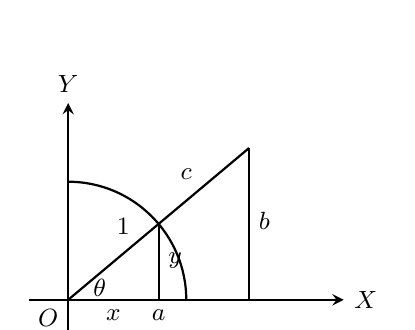
\begin{tikzpicture}[>=stealth, scale=1.0, font=\small]
  \draw[->, thick] (-0.5, 0) -- (3.5, 0) node[right] {$X$};
  \draw[->, thick] (0, -0.5) -- (0, 2.5) node[above] {$Y$};
  \draw[thick] (1.5, 0) arc (0:90:1.5);
  \coordinate (O) at (0, 0);
  \coordinate (P) at (40:1.5);
  \coordinate (BigP) at (40:3.0);
  \draw[thick] (O) -- (BigP);
  \draw[thick] (P) -- ({1.5*cos(40)}, 0);
  \draw[thick] (BigP) -- ({3.0*cos(40)}, 0);
  \node[below left] at (O) {$O$};
  \node at (0.4, 0.15) {$\theta$};
  \node[above] at (0.7, 0.7) {$1$};
  \node[above] at (1.5, 1.4) {$c$};
  \node[right] at ({1.5*cos(40)}, 0.5) {$y$};
  \node[right] at ({3.0*cos(40)}, 1.0) {$b$};
  \node[below] at ({0.5*1.5*cos(40)}, 0) {$x$};
  \node[below] at ({0.5*3.0*cos(40)}, 0) {$a$};
\end{tikzpicture}
\caption{銳角廣義與直角三角形定義一致性}
\label{fig:b3-fig2-26}
\end{figure}

(II) 從定義得知，既然 $\mathbf{r}_1$ 固定在 $OX$ 軸上，三角函數之值只依賴於終邊的位置，與它相應的 $\angle\theta$ 之旋轉經過無關；例如
\begin{align*}
\sin\frac{2\pi}{3} &= \sin\left(-\frac{4\pi}{3}\right) = \sin\left(\frac{2\pi}{3}-2\pi\right) \\
\sin\frac{2\pi}{3} &= \sin\left(\frac{2\pi}{3}+2\pi\right) = \sin\left(\frac{2\pi}{3}+4\pi\right)
\end{align*}

\begin{figure}[H]
\centering
\begin{minipage}{0.48\textwidth}
\centering
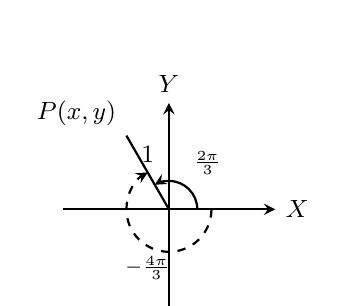
\begin{tikzpicture}[>=stealth, scale=0.9, font=\small]
  \draw[->, thick] (-1.5, 0) -- (1.5, 0) node[right] {$X$};
  \draw[->, thick] (0, -1.5) -- (0, 1.5) node[above] {$Y$};
  \coordinate (O) at (0, 0);
  \coordinate (P) at (120:1.2);
  \draw[thick] (O) -- (P) node[above left] {$P(x, y)$};
  \draw[->, thick] (0.4, 0) arc (0:120:0.4) node[midway, above right] {\scriptsize $\frac{2\pi}{3}$};
  \draw[->, thick, dashed] (0.6, 0) arc (0:-240:0.6) node[midway, below] {\scriptsize $-\frac{4\pi}{3}$};
  \node[above] at (120:0.6) {$1$};
\end{tikzpicture}
\caption{$\frac{2\pi}{3}$ 與 $-\frac{4\pi}{3}$ 同界}
\label{fig:b3-fig2-27-1}
\end{minipage}
\hfill
\begin{minipage}{0.48\textwidth}
\centering
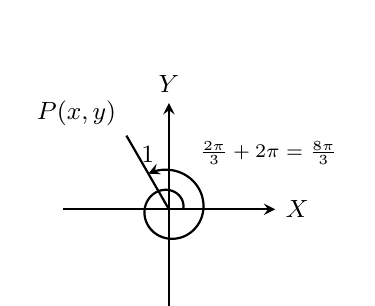
\begin{tikzpicture}[>=stealth, scale=0.9, font=\small]
  \draw[->, thick] (-1.5, 0) -- (1.5, 0) node[right] {$X$};
  \draw[->, thick] (0, -1.5) -- (0, 1.5) node[above] {$Y$};
  \coordinate (O) at (0, 0);
  \coordinate (P) at (120:1.2);
  \draw[thick] (O) -- (P) node[above left] {$P(x, y)$};
  \draw[->, thick, domain=0:480, samples=150, variable=\t]
    plot ({0.2 + 0.0008*\t)*cos(\t)}, {(0.2 + 0.0008*\t)*sin(\t)});
  \node[right] at (0.3, 0.8) {\scriptsize $\frac{2\pi}{3}+2\pi = \frac{8\pi}{3}$};
  \node[above] at (120:0.6) {$1$};
\end{tikzpicture}
\caption{$\frac{2\pi}{3}$ 與 $\frac{8\pi}{3}$ 同界}
\label{fig:b3-fig2-27-2}
\end{minipage}
\end{figure}

其實，對於任何一個三角函數 $T(t)$（$T$ 可為 $\sin, \cos, \tan, \dots\dots$ 中任何一函數）我們都有
\[ T(t) = T(t + 2n\pi);\qquad n \text{ 為任何整數.} \]
道理的關鍵在於三角函數只依賴於終邊的 $P$ 點座標成分 $x$ 與 $y$，故與 $\angle\theta$ 旋轉的經過無關. 因此三角函數是週期性的函數.

$X, Y$ 兩軸把座標平面分割為四部分，每一部分稱為一個象限，自逆時針方向數過來按次稱為第一、二、三、四象限. 常以羅馬大寫 $\mathrm{I}, \mathrm{II}, \mathrm{III}, \mathrm{IV}$ 表示，如圖 2-28.

現在我們知道三角函數的值只依賴於終邊的位置，以下便根據終邊座落的位置來看各三角函數的正負變化情形：

當 $t$ 從 0 慢慢增加，經 $\frac{\pi}{2}$，$\pi$，$\frac{3\pi}{2}$ 到 $2\pi$ 的過程中，$\sin t$ 相應地也從 0 開始增加到 1 後降落到 0 更降落到 $-1$，然後又開始增加，慢慢回復到 0. 等 $t$ 超過 $2\pi$ 後，則 $\sin t$ 又重複原來的現象. 這樣週而復始地起伏.

列表將各函數的正負變化描出，也許清楚一些.（但這表也不是用來強記的）

\begin{figure}[H]
\centering
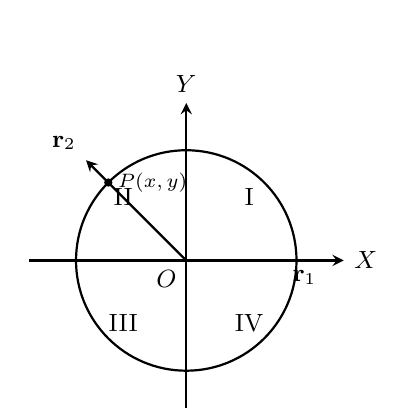
\begin{tikzpicture}[>=stealth, scale=1.0, font=\small]
  \draw[->, thick] (-2, 0) -- (2, 0) node[right] {$X$};
  \draw[->, thick] (0, -2) -- (0, 2) node[above] {$Y$};
  \draw[thick] (0, 0) circle (1.4cm);
  \node at (0.8, 0.8) {$\mathrm{I}$};
  \node at (-0.8, 0.8) {$\mathrm{II}$};
  \node at (-0.8, -0.8) {$\mathrm{III}$};
  \node at (0.8, -0.8) {$\mathrm{IV}$};
  \coordinate (O) at (0, 0);
  \coordinate (P) at (135:1.4);
  \draw[->, thick] (O) -- (135:1.8) node[above left] {$\mathbf{r}_2$};
  \fill (P) circle (1.5pt) node[right] {\scriptsize $P(x, y)$};
  \node[below] at (1.5, 0) {$\mathbf{r}_1$};
  \node[below left] at (O) {$O$};
\end{tikzpicture}
\caption{平面之四個象限}
\label{fig:b3-fig2-28}
\end{figure}

\begin{table}[H]
\centering
\small
\setlength{\tabcolsep}{3pt}
\renewcommand{\arraystretch}{1.2}
\begin{tabular}{|c|c|c|c|c|c|c|c|c|}
\hline
終邊 $\mathbf{r}_2$ 的位置 & $\mathbf{r}_2 = \vec{OX}$ & $\mathbf{r}_2 \subset \mathrm{I}^*$ & $\mathbf{r}_2 = \vec{OY}$ & $\mathbf{r}_2 \subset \mathrm{II}^*$ & $\mathbf{r}_2 = \vec{OX'}$ & $\mathbf{r}_2 \subset \mathrm{III}^*$ & $\mathbf{r}_2 = \vec{OY'}$ & $\mathbf{r}_2 \subset \mathrm{IV}^*$ \\ \hline
\shortstack{$\mathbf{r}_2$ 上 $P$ 點的座\\標 $x$ 與 $y$} & \shortstack{$x=1$\\$y=0$} & \shortstack{$x>0$\\$y>0$} & \shortstack{$x=0$\\$y=1$} & \shortstack{$x<0$\\$y>0$} & \shortstack{$x=-1$\\$y=0$} & \shortstack{$x<0$\\$y<0$} & \shortstack{$x=0$\\$y=-1$} & \shortstack{$x>0$\\$y<0$} \\ \hline
$\sin t = y$ & $0$ & $\stackrel{+}{\nearrow}$ & $1$ & $\stackrel{+}{\searrow}$ & $0$ & $\stackrel{-}{\searrow}$ & $-1$ & $\stackrel{-}{\nearrow}$ \\ \hline
$\cos t = x$ & $1$ & $\stackrel{+}{\searrow}$ & $0$ & $\stackrel{-}{\searrow}$ & $-1$ & $\stackrel{-}{\nearrow}$ & $0$ & $\stackrel{+}{\nearrow}$ \\ \hline
$\tan t = \frac{y}{x}$ & $0$ & $\stackrel{+}{\nearrow}$ & $+\infty \mid -\infty$ & $\stackrel{-}{\nearrow}$ & $0$ & $\stackrel{+}{\nearrow}$ & $+\infty \mid -\infty$ & $\stackrel{-}{\nearrow}$ \\ \hline
$\cot t = \frac{x}{y}$ & $-\infty \mid +\infty$ & $\stackrel{+}{\searrow}$ & $0$ & $\stackrel{-}{\searrow}$ & $-\infty \mid +\infty$ & $\stackrel{+}{\searrow}$ & $0$ & $\stackrel{+}{\searrow}$ \\ \hline
$\sec t = \frac{1}{x}$ & $1$ & $\stackrel{+}{\nearrow}$ & $+\infty \mid -\infty$ & $\stackrel{-}{\nearrow}$ & $-1$ & $\stackrel{-}{\searrow}$ & $-\infty \mid +\infty$ & $\stackrel{+}{\searrow}$ \\ \hline
$\csc t = \frac{1}{y}$ & $-\infty \mid +\infty$ & $\stackrel{+}{\searrow}$ & $1$ & $\stackrel{+}{\nearrow}$ & $+\infty \mid -\infty$ & $\stackrel{-}{\nearrow}$ & $-1$ & $\stackrel{-}{\searrow}$ \\ \hline
\end{tabular}
\par\vspace{3pt}
{\footnotesize (* 這裡 $\mathbf{r}_2 \subset \mathrm{I}$ 意指終邊位置落在第一象限)}
\end{table}

\textbf{註}：此表所用 $\infty$ 可以看成無意義，但其實它有深一層的意思，比如當 $\mathbf{r}_2 = \vec{OY}$ 時，在 $t = \frac{\pi}{2}$ 之點 $\tan t$ 沒有定義，但 $\tan t = \pm\infty$ 的意思是當 $t$ 增大而向 $\pi/2$ 逼近時 $\tan t$ 趨於「正無限大」，另一方面當 $t$ 減小而向 $\pi/2$ 逼近時，$\tan t$ 趨於「負無限大」（參見圖 2-30）.

從廣義三角函數的定義知在 $-\infty < t < \infty$ 之間，亦有 $\sin t$ 與 $\csc t$, $\cos t$ 與 $\sec t$, $\tan t$ 與 $\cot t$ 各對函數值互為倒數，即
\[ \sin t = \frac{1}{\csc t},\qquad \cos t = \frac{1}{\sec t},\qquad \tan t = \frac{1}{\cot t} \]
故只注意前面三個函數 $\sin t, \cos t, \tan t$ 的正負變化，便立即或可得相應的 $\csc t, \sec t, \cot t$ 的正負變化情形.

\begin{figure}[H]
\centering
\begin{tikzpicture}[scale=0.9, font=\small]
  \draw[thick] (-2, 0) -- (2, 0);
  \draw[thick] (0, -1.5) -- (0, 1.5);
  \node at (1, 1) {\shortstack{$\mathrm{I}$\\全 $+$}};
  \node at (-1, 1) {\shortstack{$\mathrm{II}$\\$\sin t = +$\\$\csc t = +$}};
  \node at (-1, -0.8) {\shortstack{$\mathrm{III}$\\$\tan t = +$\\$\cot t = +$}};
  \node at (1, -0.8) {\shortstack{$\mathrm{IV}$\\$\cos t = +$\\$\sec t = +$}};
\end{tikzpicture}
\caption{各象限三角函數正負符號分佈}
\end{figure}

(III) 一質點 $P(x, y)$ 在單位圓上，自 $(1, 0)$ 點出發，以單位角速度〔即每單位時間走一弧度的等速轉動〕沿逆時針方向運動，則在 $t$ 時刻，$P$ 的位置正好落在張角 $\angle\theta$ 之角度為 $t$ 的地方（為什麼？留作習題）故
\[ \sin t = y \quad\text{與}\quad \cos t = x \]
正好描寫這質點 $P(x, y)$ 分別在 $\vec{OY}$ 軸與在 $\vec{OX}$ 軸上的投影. 從表二可以描出 $u = \sin t$ 的函數圖形約略是如下的波形：

\begin{figure}[H]
\centering
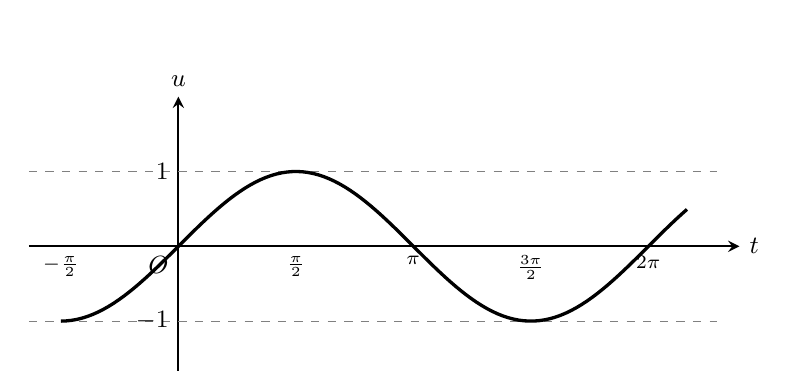
\begin{tikzpicture}[>=stealth, scale=0.95, font=\small]
  \draw[->, thick] (-2, 0) -- (7.5, 0) node[right] {$t$};
  \draw[->, thick] (0, -1.8) -- (0, 2) node[above] {$u$};

  \draw[dashed, gray] (-2, 1) -- (7.2, 1);
  \draw[dashed, gray] (-2, -1) -- (7.2, -1);
  \node[left] at (0, 1) {$1$};
  \node[left] at (0, -1) {$-1$};
  \node[below left] at (0, 0) {$O$};

  \draw[very thick, domain=-1.57:6.8, samples=120] plot (\x, {sin(\x r)});

  \node[below] at (-1.57, 0) {\scriptsize $-\frac{\pi}{2}$};
  \node[below] at (1.57, 0) {\scriptsize $\frac{\pi}{2}$};
  \node[below] at (3.14, 0) {\scriptsize $\pi$};
  \node[below] at (4.71, 0) {\scriptsize $\frac{3\pi}{2}$};
  \node[below] at (6.28, 0) {\scriptsize $2\pi$};
\end{tikzpicture}
\caption{$u = \sin t$ 的函數圖形}
\label{fig:b3-fig2-29}
\end{figure}

至於 $u = \cos t$ 的函數圖形留當習題.

(IV) 參照表二中三角函數的變化情形我們畫出 $u = \tan t$ 與 $u = \sec t$ 的函數圖形（而將 $u = \cot t$ 與 $u = \csc t$ 的圖形留當習題）.

\begin{figure}[H]
\centering
\begin{tikzpicture}[>=stealth, scale=0.9, font=\small]
  \draw[->, thick] (-3.8, 0) -- (7, 0) node[right] {$t$};
  \draw[->, thick] (0, -3) -- (0, 3) node[above] {$u$};

  % Asymptotes
  \foreach \x in {-1.57, 1.57, 4.71} {
    \draw[dashed, gray] (\x, -2.8) -- (\x, 2.8);
  }

  % Tangent branches
  \draw[very thick, domain=-3.6:-1.7, samples=60] plot (\x, {tan(\x r)});
  \draw[very thick, domain=-1.35:1.35, samples=60] plot (\x, {tan(\x r)});
  \draw[very thick, domain=1.75:4.5, samples=60] plot (\x, {tan(\x r)});
  \draw[very thick, domain=4.9:6.6, samples=60] plot (\x, {tan(\x r)});

  \node[below] at (-3.14, 0) {\scriptsize $-\pi$};
  \node[below] at (-1.57, 0) {\scriptsize $-\frac{\pi}{2}$};
  \node[below left] at (0, 0) {$O$};
  \node[below] at (1.57, 0) {\scriptsize $\frac{\pi}{2}$};
  \node[below] at (3.14, 0) {\scriptsize $\pi$};
  \node[below] at (4.71, 0) {\scriptsize $\frac{3\pi}{2}$};
  \node[below] at (6.28, 0) {\scriptsize $2\pi$};
\end{tikzpicture}
\caption{$u = \tan t$ 的圖形}
\label{fig:b3-fig2-30}
\end{figure}

\begin{figure}[H]
\centering
\begin{tikzpicture}[>=stealth, scale=0.9, font=\small]
  \draw[->, thick] (-3.8, 0) -- (7, 0) node[right] {$t$};
  \draw[->, thick] (0, -3) -- (0, 3) node[above] {$u$};

  \draw[dashed, gray] (-3.8, 1) -- (6.8, 1);
  \draw[dashed, gray] (-3.8, -1) -- (6.8, -1);

  % Asymptotes
  \foreach \x in {-1.57, 1.57, 4.71} {
    \draw[dashed, gray] (\x, -2.8) -- (\x, 2.8);
  }

  % Secant branches
  \draw[very thick, domain=-1.3:1.3, samples=50] plot (\x, {1/cos(\x r)});
  \draw[very thick, domain=1.85:4.4, samples=50] plot (\x, {1/cos(\x r)});
  \draw[very thick, domain=4.95:6.8, samples=50] plot (\x, {1/cos(\x r)});

  \node[below] at (-3.14, 0) {\scriptsize $-\pi$};
  \node[below] at (-1.57, 0) {\scriptsize $-\frac{\pi}{2}$};
  \node[below left] at (0, 0) {$O$};
  \node[below] at (1.57, 0) {\scriptsize $\frac{\pi}{2}$};
  \node[below] at (3.14, 0) {\scriptsize $\pi$};
  \node[below] at (4.71, 0) {\scriptsize $\frac{3\pi}{2}$};
  \node[below] at (6.28, 0) {\scriptsize $2\pi$};
\end{tikzpicture}
\caption{$u = \sec t$ 的圖形}
\label{fig:b3-fig2-31}
\end{figure}

\phantomsection\label{note:b3-ch2-p41-ex4-typo}%
\begin{example}
已知 $\alpha = 1230^\circ$，求 $\sin\alpha, \cos\alpha, \tan\alpha$\footnote{【校訂註】原書題幹印作「$\text{tara }\alpha$」，實為「$\tan\alpha$」之印刷訛字。正文照原印字樣錄入並在此校記。} 之值.
\end{example}

\begin{proof}[解]
$1230^\circ = 3 \times 360^\circ + 150^\circ = 3 \times 2\pi + \frac{5\pi}{6}$（弧度）

\phantomsection\label{note:b3-ch2-p41-ref-fig31}%
依定義取 $\angle(\theta; \mathbf{r}_1, \mathbf{r}_2)$ 使 $\mathbf{r}_1$ 與 $OX$ 軸重疊，則終邊 $\mathbf{r}_2$ 落在第二象限 $\mathrm{II}$（如圖 2-31\footnote{【校訂註】原書行文稱「如圖 2-31」，圖 2-31 實為前文割線函數圖形，本例題之旋轉角終邊示意圖印於次頁圖 2-32。正文保留原書字樣。}）

\begin{enumerate}[label=(\roman*), leftmargin=2.5em]
  \item $\sin 1230^\circ = \sin\left(3\times 2\pi + \frac{5\pi}{6}\right) = \sin\frac{5\pi}{6} = y = \frac{1}{2}$
  \item $\cos 1230^\circ = \cos\left(3\times 2\pi + \frac{5\pi}{6}\right) = \cos\frac{5\pi}{6} = x = -\frac{\sqrt{3}}{2}$
  \item $\tan 1230^\circ = \tan\left(3\times 2\pi + \frac{5\pi}{6}\right) = \tan\frac{5\pi}{6} = \frac{y}{x} = -\frac{1}{\sqrt{3}} \qedhere$
\end{enumerate}
\end{proof}

\begin{figure}[H]
\centering
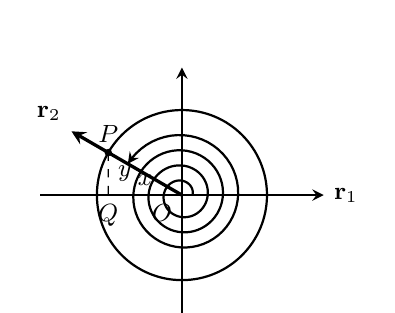
\begin{tikzpicture}[>=stealth, scale=0.9, font=\small]
  \draw[->, thick] (-2, 0) -- (2, 0) node[right] {$\mathbf{r}_1$};
  \draw[->, thick] (0, -1.8) -- (0, 1.8);
  \draw[thick] (0, 0) circle (1.2cm);
  \coordinate (O) at (0, 0);
  \coordinate (P) at (150:1.2);
  \draw[->, very thick] (O) -- (150:1.8) node[above left] {$\mathbf{r}_2$};
  \fill (P) circle (1.5pt) node[above] {$P$};
  \draw[dashed] (P) -- ({1.2*cos(150)}, 0) node[below] {$Q$};
  \draw[->, thick, domain=0:1230, samples=200, variable=\t]
    plot ({0.15 + 0.0006*\t)*cos(\t)}, {(0.15 + 0.0006*\t)*sin(\t)});
  \node[below left] at (O) {$O$};
  \node[above] at ({0.5*1.2*cos(150)}, 0) {$x$};
  \node[right] at ({1.2*cos(150)}, 0.3) {$y$};
\end{tikzpicture}
\caption{$1230^\circ$ 旋轉角終邊分析}
\label{fig:b3-fig2-32}
\end{figure}

\begin{example}
若 $\cot t \cos t > 0$，則相應的 $\angle\theta$ 之終邊 $\mathbf{r}_2$ 應落在第幾象限？
\end{example}

\begin{proof}[解]
$\cot t \cos t > 0 \iff \cot t > 0, \cos t > 0$ 或 $\cot t < 0, \cos t < 0$.

故 $\mathbf{r}_2$ 落在第一或第二象限. \qedhere
\end{proof}

\subsubsection*{作業 8}
\begin{enumerate}[label=\roman*), leftmargin=2.5em]
  \item 求下列各三角函數值：
  \[ \cot 150^\circ,\quad \sin 225^\circ,\quad \tan(-570^\circ),\quad \cos\frac{20}{3}\pi \]
  \item 若 $\cos t < 0, \tan t > 0$，則相應的 $\angle\theta$ 之終邊 $\mathbf{r}_2$ 應落在第幾象限？
  \item 點 $(\cot(-4), \sec(-4))$ 應落在第幾象限？
\end{enumerate}

\subsection*{習題 2-2}

\begin{enumerate}[label=\arabic*., leftmargin=2em]
  \item 設一質點 $P(x, y)$ 在單位圓上，自 $(1, 0)$ 出發，以角速度 $w=1$（弧度/秒）沿逆時針方向運動，試證在 $t$ 秒時，$P$ 的位置正好落在張角 $\angle\theta$ 之角度為 $t$ 的地方.
  \item 描出 $u = \cos t$ 的圖形.
  \item 描出 $u = \cot t$ 與 $u = \csc t$ 的圖形.
  \item 試求函數曲線 $u = \sin t$ 與 $u = \cos t$ 的交點.
  \item 利用 $t \to 3t \to 3t-\frac{\pi}{2} \to \sin(3t-\frac{\pi}{2}) \to 2\sin(3t-\frac{\pi}{2})$ 這一系列函數的合成函數描出 $u = 2\sin(3t-\frac{\pi}{2})$ 之函數圖形.
  \item 試描出 $u = \sin t + \cos t$ 之函數圖形.
  \item 利用三角函數寫出單位圓內接正六邊形的周長及面積.
  \item[*] 圖示下列各式：
  \begin{enumerate}[label=(\roman*), leftmargin=2.5em]
    \item $y = |\sin t|$ \qquad (ii) $y = \cos t - |\cos t|$ \qquad (iii) $y = \csc t + |\csc t|$
  \end{enumerate}
  \item 已知 $0 < \theta < \frac{\pi}{2}$ 則 $\sin\theta < \theta$ 試證之.
  \item 圖 2-34 中，點 $P$ 之座標為何？
  \begin{flushright}
  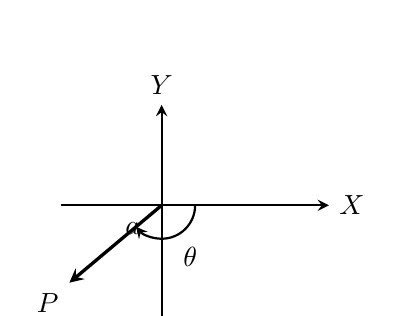
\begin{tikzpicture}[>=stealth, scale=0.85, baseline=(current bounding box.center)]
    \draw[->, thick] (-1.5, 0) -- (2.5, 0) node[right] {$X$};
    \draw[->, thick] (0, -1.8) -- (0, 1.5) node[above] {$Y$};
    \coordinate (O) at (0, 0);
    \coordinate (P) at (-140:1.8);
    \draw[->, very thick] (O) -- (P) node[below left] {$P$};
    \draw[->, thick] (0.5, 0) arc (0:-140:0.5) node[midway, below right] {$\theta$};
    \node[above right] at (-140:0.9) {$a$};
  \end{tikzpicture}
  \end{flushright}
  \item 假設我們已經知道
  \begin{enumerate}[label=(\roman*), leftmargin=2.5em]
    \item $-1 \le \sin x \le 1$
    \item 當 $x > 0$，滿足 $\sin x = 0$ 之點為 $\pi, 2\pi, 3\pi, \dots\dots$，（稱為 $\sin x$ 之零點）\\
    滿足 $\sin x = +1$ 之點為 $\frac{\pi}{2}, 2\pi+\frac{\pi}{2}, 4\pi+\frac{\pi}{2}, \dots\dots$（稱為 $\sin x$ 之峯點）\\
    滿足 $\sin x = -1$ 之點為 $\frac{3\pi}{2}, 2\pi+\frac{3\pi}{2}, 4\pi+\frac{3\pi}{2}, \dots\dots$（稱為 $\sin x$ 之谷點）
  \end{enumerate}
  我們便概略繪得 $\sin x$ 之函數圖形如下：
  \begin{center}
  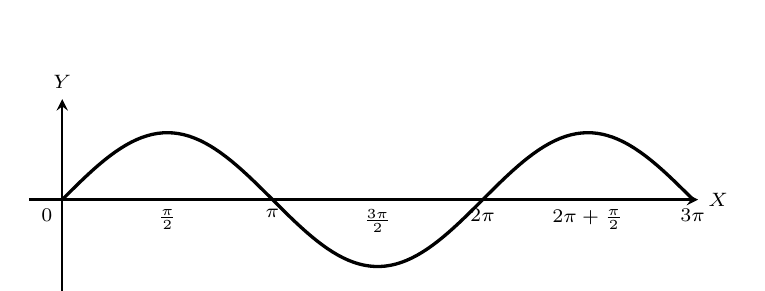
\begin{tikzpicture}[>=stealth, scale=0.85, font=\scriptsize]
    \draw[->, thick] (-0.5, 0) -- (9.5, 0) node[right] {$X$};
    \draw[->, thick] (0, -1.5) -- (0, 1.5) node[above] {$Y$};
    \draw[domain=0:9.42, samples=120, very thick] plot (\x, {sin(\x r)});
    \node[below left] at (0, 0) {$0$};
    \node[below] at (1.57, 0) {$\frac{\pi}{2}$};
    \node[below] at (3.14, 0) {$\pi$};
    \node[below] at (4.71, 0) {$\frac{3\pi}{2}$};
    \node[below] at (6.28, 0) {$2\pi$};
    \node[below] at (7.85, 0) {$2\pi+\frac{\pi}{2}$};
    \node[below] at (9.42, 0) {$3\pi$};
  \end{tikzpicture}
  \end{center}
  \begin{enumerate}[label=(\alph*), leftmargin=2.5em]
    \item 證明：$x \ne 0$; $-1 \le \sin\frac{1}{x} \le 1$
    \item 求 $\sin\frac{1}{x}$ 的零點，峯點、谷點.
    \item 並仿上述大略畫出 $\sin\frac{1}{x}$ 的圖形.
  \end{enumerate}
\end{enumerate}

\subsection{一些簡易的恒等式}
\label{subsec:b3-2-3}

本節將沿用 §2-2 的所有符號.

三角函數之間有各種關係，本節只提一些簡易的恆等式，以供本冊之用，其餘目前用不著的〔像和角公式：即將 $\sin(t_1 + t_2)$ 表成 $t_1$ 與 $t_2$ 的三角函數，如 $\sin t_1, \cos t_2$ 等的公式〕暫時放在一邊，因為它們的一般導引方法是利用圖解，依賴圖解，不僅先天上難具一般性〔如導引和角公式時，要取 $t_1, t_2$ 使相應角度 $\overline{\theta_1}, \overline{\theta_2}$ 落到那一象限呢？〕，而導引的過程也難以表現它的要點. 我們這樣做更重要的原因是：我們現在講述三角函數，只為它一些簡易性質將在本冊各種問題的處理需用，中心並不放在三角函數本身. 我們希望能很快地能跳過這段三角函數的講述，在作過測量的應用後，迅速轉入本冊的主題：向量幾何與座標幾何的代數轉化！不願現在就陷入三角函數傳統技巧的故紙堆裏. 到了第三章，在向量內積引進來後還要利用它導引和角公式. 我們無意要把三角函數作為一個獨立的題材來講述. 相反地，我們要隨著幾何與代數間的轉化這一主題的需要，和可用來簡捷處理三角函數的各項工具（如向量、複數）的逐次發展，來一步步引出三角函數的各項有用的性質.

\begin{proposition}
對下列函數有定義的任意實數 $t$，我們有下列恆等式
\begin{align*}
\sin^2 t + \cos^2 t &= 1,\qquad 1 + \tan^2 t = \sec^2 t \\
1 + \cot^2 t &= \csc^2 t
\end{align*}
\end{proposition}

\begin{proof}
其實這組恆等式就是畢氏定理的化身：
\[ \sin^2 t + \cos^2 t = y^2 + x^2 = \overline{OP}^2 = 1 \quad\text{〔符號沿用 §2-2 的定義〕} \]
\[ 1 + \tan^2 t = 1 + \frac{y^2}{x^2} = \frac{x^2 + y^2}{x^2} = \frac{1}{x^2} = \sec^2 t \]
\[ 1 + \cot^2 t = 1 + \frac{x^2}{y^2} = \frac{y^2 + x^2}{y^2} = \frac{1}{y^2} = \csc^2 t \qedhere \]
\end{proof}

\begin{proposition}[負角公式]
我們有
\begin{align*}
\sin t &= -\sin(-t) \\
\cos t &= \cos(-t) \\
\tan t &= -\tan(-t)
\end{align*}
\end{proposition}

\begin{proof}
由三角函數的定義知其符號（值）只與其所對應的廣義有向角的終邊的位置有關. 今對實數 $t$，取其對應角的始邊為 $OX$，若終邊在第 $\mathrm{I}$ 象限，則對應於 $-t$ 的角的終邊會落在第 $\mathrm{IV}$ 象限，而若終邊在第 $\mathrm{II}$ 象限，則對應於 $-t$ 的角的終邊在第 $\mathrm{III}$ 象限，調換 $\mathrm{I}$ 與 $\mathrm{IV}$ 或 $\mathrm{II}$ 與 $\mathrm{III}$ 的位置結果亦同. 今若各在其終邊上取點 $P(x, y), Q(x', y')$，則有 $x = x', y = -y'$（為什麼，請自證）.

今
\begin{align*}
\sin t &= y,\quad \sin(-t) = y' \\
\cos t &= x,\quad \cos(-t) = x' \\
\tan t &= y/x,\quad \tan(-t) = y'/x'
\end{align*}
故得證.
\end{proof}

在 §2-28 甲的作業裏，我們已要同學們算幾個特別角的三角函數值，今再整理一表，列表如下：

\begin{proposition}
\begin{center}
\renewcommand{\arraystretch}{1.3}
\begin{tabular}{|c|c|c|c|}
\hline
$t$ 值 & $\frac{\pi}{6}$ & $\frac{\pi}{4}$ & $\frac{\pi}{3}$ \\ \hline
$\sin t$ & $\frac{1}{2}$ & $\frac{1}{\sqrt{2}}$ & $\frac{\sqrt{3}}{2}$ \\ \hline
$\cos t$ & $\frac{\sqrt{3}}{2}$ & $\frac{1}{\sqrt{2}}$ & $\frac{1}{2}$ \\ \hline
$\tan t$ & $\frac{1}{\sqrt{3}}$ & $1$ & $\sqrt{3}$ \\ \hline
\end{tabular}
\end{center}
\end{proposition}

\begin{example}
已知 $\sin\theta = \frac{8}{17}$, $\frac{\pi}{2} < \theta < \pi$，求 $\cos\theta, \tan\theta$ 之值.
\end{example}

\begin{proof}[解]
由畢氏定理知 $\sin\theta$ 與 $\cos\theta$ 間存在恆等關係：
\[ \sin^2\theta + \cos^2\theta = 1 \]
故 $\cos\theta = \pm\sqrt{1 - \left(\frac{8}{17}\right)^2} = \pm\frac{15}{17}$，因 $\theta$ 在第二象限 $\cos\theta < 0$ 故取負值，得 $\cos\theta = -\frac{15}{17}$.

另一方面 $\tan\theta = \frac{\sin\theta}{\cos\theta} = -\frac{8}{15}$. \qedhere
\end{proof}

\subsubsection*{作業 9}
\begin{enumerate}[label=\roman*), leftmargin=2.5em]
  \item 已知 $\tan\theta = -\frac{2}{3}$, $\frac{3}{2}\pi < \theta < 2\pi$，求 $\sin\theta, \cos\theta$ 之值.
  \item 試證 $\sin(\pi-\theta) = \sin\theta$, $\cos(\pi-\theta) = -\cos\theta$, $\tan(\pi-\theta) = -\tan\theta$.〔想法如命題 6〕
\end{enumerate}

\begin{example}
設 $\sin(-100^\circ) = k$，試以 $k$ 表出 $\cot 260^\circ$.
\end{example}

\begin{proof}[解]
要用正弦表出 $\cot 260^\circ$，先考慮 $\cot$ 與 $\sin$ 和 $\cos$ 的關係
\[ \cot 260^\circ = \frac{\cos 260^\circ}{\sin 260^\circ} \]
但 $\sin 260^\circ = \sin(360^\circ - 100^\circ) = \sin(-100^\circ) = k$.

且 $\cos 260^\circ = \cos(360^\circ - 100^\circ) = \cos(-100^\circ) = \cos 100^\circ = -\sqrt{1 - \sin^2 100^\circ} = -\sqrt{1 - k^2}$.

故 $\cot 260^\circ = -\frac{\sqrt{1 - k^2}}{k}$. \qedhere
\end{proof}

\begin{proposition}[銳角的倍角公式]
設 $0 < t < \frac{\pi}{2}$，則
\begin{align*}
\sin 2t &= 2\sin t\cos t \\
\cos 2t &= 1 - 2\sin^2 t = 2\cos^2 t - 1
\end{align*}
\end{proposition}

\begin{proof}
取一直角三角形 $\triangle QOP$，使 $\angle QOP$ 的角度為 $t$，且斜邊 $\overline{OP} = 1$，則
\[ \overline{PQ} = \sin t,\quad \overline{OQ} = \cos t. \]
取 $P$ 對於直線 $OQ$ 的鏡像點 $P'$，自 $P$ 引 $OP'$ 的垂線 $PR$，則
\[ \overline{PR} = \sin 2t,\quad \overline{OR} = \cos 2t. \]
因 $\angle RP'P$ 之角度為 $\frac{\pi}{2}-t$，故
\[ \sin\left(\frac{\pi}{2}-t\right) = \frac{\overline{PR}}{\overline{PP'}} = \frac{\sin 2t}{2\sin t} \]
而左端 $\sin\left(\frac{\pi}{2}-t\right) = \cos t$，故得 $\sin 2t = 2\sin t\cos t$.

另一方面，$\overline{OR} + \overline{RP'} = \overline{OP'} = 1$，但
\[ \frac{\overline{RP'}}{\overline{PP'}} = \cos\left(\frac{\pi}{2}-t\right) = \sin t \]
故 $\overline{RP'} = \overline{PP'}\sin t = 2\sin^2 t$.

故 $\cos 2t + 2\sin^2 t = 1$，故 $\cos 2t = 1 - 2\sin^2 t$.

又 $\sin^2 t = 1 - \cos^2 t$，故 $\cos 2t = 1 - 2\sin^2 t = 1 - 2 + 2\cos^2 t = 2\cos^2 t - 1$.
\end{proof}

\begin{figure}[H]
\centering
\begin{tikzpicture}[>=stealth, scale=1.2, font=\small]
  \coordinate (O) at (0, 0);
  \coordinate (P) at (25:4);
  \coordinate (Pprime) at (-25:4);
  \coordinate (Q) at ({4*cos(25)}, 0);

  \draw[thick] (O) -- (Q);
  \draw[very thick] (O) -- (P) node[above right] {$P$};
  \draw[very thick] (O) -- (Pprime) node[below right] {$P'$};
  \draw[thick] (P) -- (Pprime);
  \draw (Q) rectangle ++(-0.2, 0.2);

  % PR perpendicular to OP'
  \coordinate (R) at ($(O)!{4*cos(50)}!(Pprime)$);
  \draw[thick] (P) -- (R);
  \draw[rotate=-25] (R) rectangle ++(-0.2, 0.2);

  \node[left] at (O) {$O$};
  \node[above] at (Q) {$Q$};
  \node[below left] at (R) {$R$};

  \node at (0.8, 0.15) {$t$};
  \node at (0.8, -0.15) {$t$};
  \node[above left] at (2, 0.8) {$1$};
  \node[above] at ($(P)!0.5!(Pprime)$) {};
  \node[right] at ($(R)!0.5!(Pprime)$) {\scriptsize $\frac{\pi}{2}-t$};
\end{tikzpicture}
\caption{倍角公式鏡像幾何證明}
\label{fig:b3-fig2-35}
\end{figure}

容易驗證當 $t = \frac{\pi}{4}$ 時，上命題亦成立. 至於當 $\frac{\pi}{4} < t < \frac{\pi}{2}$，可取 $0 < s < \frac{\pi}{4}$，使 $s + t = \frac{\pi}{2}$.

利用作業 9 (ii)
\begin{align*}
\sin 2t &= \sin 2\left(\frac{\pi}{2}-s\right) = \sin(\pi - 2s) = \sin 2s \\
\cos 2t &= \cos 2\left(\frac{\pi}{2}-s\right) = \cos(\pi - 2s) = -\cos 2s
\end{align*}
將命題 8 代入上式，再由銳角的餘角公式（命題 3）可得
\begin{align*}
\sin 2t &= 2\sin t\cos t \\
\cos 2t &= 2\cos^2 t - 1 = 1 - 2\sin^2 t,\quad \frac{\pi}{4} < t < \frac{\pi}{2}.
\end{align*}
綜合上述討論可知上式對所有 $0 < t < \frac{\pi}{2}$ 皆成立，此即正弦、餘弦的倍角公式.

事實上，這個倍角公式，對所有實數 $t$ 均成立，它的導引是以後在第三章利用向量內積處理和角公式的特殊情形.

\subsubsection*{作業 10}
\begin{enumerate}[label=\roman*), leftmargin=2.5em]
  \item 求 $\sin 15^\circ, \cos\frac{\pi}{12}, \sin\frac{\pi}{24}, \cos 22.5^\circ$ 之值.
  \item（半角公式）倍角公式告訴我們若知 $t$ 的正弦、餘弦，可求 $2t$ 的正弦、餘弦. 反過來，設已知 $t$ 的正弦、餘弦，試求 $\frac{t}{2}$ 的正弦、餘弦.
\end{enumerate}

\begin{example}
設 $\sin\theta - \cos\theta = \sqrt{2}$ 求 $\sin 2\theta$ 之值.
\end{example}

\begin{proof}[解]
$\because\quad \sin\theta - \cos\theta = \sqrt{2}$

平方之後：$\sin^2\theta - 2\sin\theta\cos\theta + \cos^2\theta = 2$

由命題 5 得：$1 - 2\sin\theta\cos\theta = 2$
\[ \therefore\quad \sin 2\theta = 2\sin\theta\cos\theta = -1 \qedhere \]
\end{proof}

\begin{example}
試證 $\sin 2t = \frac{2\tan t}{1 + \tan^2 t}$, $0 < t < \frac{\pi}{2}$.
\end{example}

\begin{proof}[證明]
\[ \text{右式} = \frac{2\tan t}{1 + \tan^2 t} = \frac{2\tan t}{\sec^2 t} = 2\frac{\sin t}{\cos t}\cos^2 t = 2\sin t\cos t \]
由正弦倍角公式知：左式 = 右式，故得證.
\end{proof}

\subsubsection*{作業 11}
\begin{enumerate}[label=\roman*), leftmargin=2.5em]
  \item 設 $\sin\alpha + \cos\alpha = \frac{1}{5}$, $0 < \alpha < \frac{\pi}{2}$. 求 $\sin 2\alpha, \sin\alpha, \cos\alpha, \sin\frac{\alpha}{2}$ 之值.
  \item 證明 $\cos 2t = \cos^2 t - \sin^2 t = \frac{1 - \tan^2 t}{1 + \tan^2 t}$.
\end{enumerate}

\subsection*{習題 2-3}

\begin{enumerate}[label=\arabic*., leftmargin=2em]
  \item 試求下列各值：
  \begin{enumerate}[label=(\roman*), leftmargin=2.5em]
    \item $\sin\frac{\pi}{6} + \tan\frac{\pi}{4}$ \qquad (ii) $\cot\frac{\pi}{4} + \cos\frac{\pi}{3}$
    \item[(iii)] $\sin\frac{\pi}{6}\cos\frac{\pi}{3} + \cos\frac{\pi}{6}\sin\frac{\pi}{3}$ \qquad (iv) $\cos\frac{\pi}{6}\cos\frac{\pi}{3} - \sin\frac{\pi}{6}\sin\frac{\pi}{3}$
    \item[(v)] $\sec\frac{\pi}{6},\; \sec\frac{\pi}{3},\; \sec\frac{\pi}{2}$.
  \end{enumerate}
  \item 試求 $\cos\frac{\pi}{8}$ 及 $\sin\frac{\pi}{8}$, $\cos\frac{\pi}{16}$ 及 $\sin\frac{\pi}{16}$.
  \item 試求單位圓內接正八邊形之周長及面積.
  \item[*] 試求單位圓內接正十六邊形之周長及面積.
  \item $\triangle ABC$ 中 $AD$ 為 $BC$ 邊上垂線，$\angle B, \angle C$ 之角度分別為 $\beta, \gamma$，已知 $\overline{BC} = a$，試以 $a, \beta, \gamma$ 表高 $\overline{AD}$.\\
  〔提示：分別根據 $\triangle ABD, \triangle ACD$ 考慮 $\beta$ 與 $\gamma$ 之正切，即 $\overline{BD} = \frac{\overline{AD}}{\tan\beta}, \overline{CD} = \frac{\overline{AD}}{\tan\gamma}$〕
  \begin{flushright}
  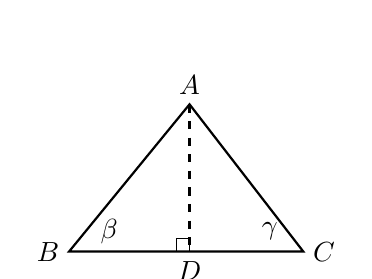
\begin{tikzpicture}[>=stealth, scale=0.85, baseline=(current bounding box.center)]
    \coordinate (B) at (0, 0);
    \coordinate (D) at (1.8, 0);
    \coordinate (C) at (3.5, 0);
    \coordinate (A) at (1.8, 2.2);
    \draw[thick] (B) -- (C) -- (A) -- cycle;
    \draw[dashed, thick] (A) -- (D);
    \draw (D) rectangle ++(-0.2, 0.2);
    \node[left] at (B) {$B$};
    \node[right] at (C) {$C$};
    \node[below] at (D) {$D$};
    \node[above] at (A) {$A$};
    \node at (0.6, 0.3) {$\beta$};
    \node at (3.0, 0.3) {$\gamma$};
  \end{tikzpicture}
  \end{flushright}
  \item 試證
  \begin{enumerate}[label=(\roman*), leftmargin=2.5em]
    \item $2\csc t = \frac{\sin t}{1 + \cos t} + \frac{1 + \cos t}{\sin t}$
    \item $\sec^2 t \csc^2 t = \sec^2 t + \csc^2 t$.
  \end{enumerate}
  \item 試簡化下列諸函數值：
  \begin{enumerate}[label=(\roman*), leftmargin=2.5em]
    \item $\sin t\sec t\cot t$
    \item $\sin^2 t(1 + \cot^2 t)$
    \item $(\sin t + \cos t)^2 + (\sin t - \cos t)^2$
    \item $\tan t + \frac{\cos t}{1 + \sin t}$.
  \end{enumerate}
  \item 已知 $\sin\theta = \frac{5}{13}$, $\angle\theta$ 之終邊在第二象限且 $0 \le \theta < \pi$，試求下列各函數值：
  \[ \cos\theta,\; \tan\theta,\; \cos\frac{\theta}{2},\; \sin\frac{\theta}{2} \]
  又 $\theta$ 值若不限制在 $0$ 與 $\pi$ 之間，只知 $\angle\theta$ 之終邊在第二象限，則上述所求各函數值是否唯一確定？可得那些新值？
  \item 
  \begin{enumerate}[label=(\roman*), leftmargin=2.5em]
    \item 若有一質點在單位圓上作等速（圓周）運動，若取一直角座標系 $(O; X, Y)$ 原點 $O$ 在單位圓圓心，且知 $\vec{OX}$ 到 $\vec{OP}$ 的轉角為 $\theta$，如本圖，則 $P$ 點的座標應為 $(\quad,\quad)$.
    \item 如果點 $P$ 在 $t=0$ 時刻從 $(1, 0)$ 位置依反時計方向，繞圓旋轉而知每繞一圈需時 1.2 秒（稱 1.2 秒為週期），問 20 秒後 $P$ 點的位置，試自行繪圖.
    \item 這樣的質點在單位圓上做等速運動時，它在 $Y$ 軸上（或 $X$ 軸上）的投影成了一個上下起伏（或左右擺動）的所謂\textbf{簡諧運動}，而由虎克定律可以推知彈簧的振動為一簡諧運動.
  \end{enumerate}
  \begin{center}
  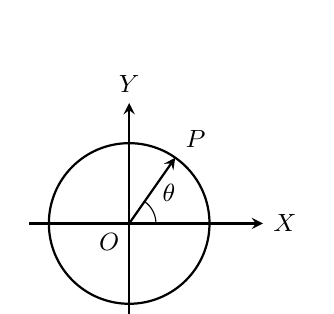
\begin{tikzpicture}[>=stealth, scale=0.85, font=\small]
    \draw[->, thick] (-1.5, 0) -- (2, 0) node[right] {$X$};
    \draw[->, thick] (0, -1.5) -- (0, 1.8) node[above] {$Y$};
    \draw[thick] (0, 0) circle (1.2cm);
    \coordinate (O) at (0, 0);
    \coordinate (P) at (55:1.2);
    \draw[->, thick] (O) -- (P) node[above right] {$P$};
    \draw (0.4, 0) arc (0:55:0.4) node[midway, above right] {$\theta$};
    \node[below left] at (O) {$O$};
  \end{tikzpicture}
  \end{center}
  試利用 (i), (ii) 所述，加以推廣，求彈簧的振動如下：將彈簧的一個端點固定使其鉛垂懸掛，而 $P$ 為另一端點設彈簧上下振動時，$P$ 點振動的幅度為 $\ell$（見圖）且 $t=a$ 時 $P$ 剛過平衡位置（$AB$ 中點，設之為 $y=0$）而週期為 $\lambda$，則 $t$ 時刻 $P$ 點的位置 $y$ 為何？
  \begin{center}
  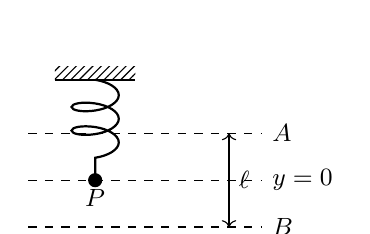
\begin{tikzpicture}[scale=0.85, font=\small]
    % Support ceiling
    \fill[pattern=north east lines] (-0.6, 2) rectangle (0.6, 2.2);
    \draw[thick] (-0.6, 2) -- (0.6, 2);
    % Spring
    \draw[thick, decoration={coil, aspect=0.4, segment length=3mm, amplitude=3mm}, decorate] (0, 2) -- (0, 0.5);
    \fill (0, 0.5) circle (3pt) node[below] {$P$};

    % Equilibrium and amplitude markers
    \draw[dashed] (-1, 0.5) -- (2.5, 0.5) node[right] {$y=0$};
    \draw[dashed] (-1, 1.2) -- (2.5, 1.2) node[right] {$A$};
    \draw[dashed] (-1, -0.2) -- (2.5, -0.2) node[right] {$B$};
    \draw[<->] (2, -0.2) -- (2, 1.2) node[midway, right] {$\ell$};
  \end{tikzpicture}
  \end{center}
\end{enumerate}

\subsection{一些幾何上量的定理}
\label{subsec:b3-2-4}

在這一節裏，我們運用直觀幾何，引入一些以後有用的幾何上的量的定理. 國中時已證知\textbf{畢氏定理}（或稱勾股弦定理）：

「直角三角形斜邊的平方等於其他兩邊的平方和.」如用式子表示，得
\begin{equation}
c^2 = a^2 + b^2 \label{eq:b3-pythagoras}
\end{equation}
其中 $c$ 表斜邊，$a, b$ 為兩直角邊. 這個式子是第一章所提過的座標幾何中根據座標量度長度的基礎. 例如：設座標系為 $(O; X, Y)$ 則任一點 $P(x, y)$ 到原點 $O$ 的距離，根據畢氏定理正好是 $\sqrt{x^2 + y^2}$.

\begin{figure}[H]
\centering
\begin{minipage}{0.48\textwidth}
\centering
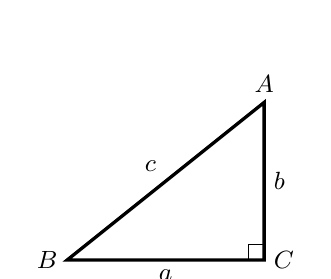
\begin{tikzpicture}[scale=1.0, font=\small]
  \coordinate (C) at (2.5, 0);
  \coordinate (B) at (0, 0);
  \coordinate (A) at (2.5, 2);
  \draw[very thick] (B) -- (C) -- (A) -- cycle;
  \draw (C) rectangle ++(-0.2, 0.2);
  \node[left] at (B) {$B$};
  \node[right] at (C) {$C$};
  \node[above] at (A) {$A$};
  \node[below] at (1.25, 0) {$a$};
  \node[right] at (2.5, 1) {$b$};
  \node[above left] at (1.25, 1) {$c$};
\end{tikzpicture}
\caption{直角三角形畢氏定理}
\label{fig:b3-fig2-37}
\end{minipage}
\hfill
\begin{minipage}{0.48\textwidth}
\centering
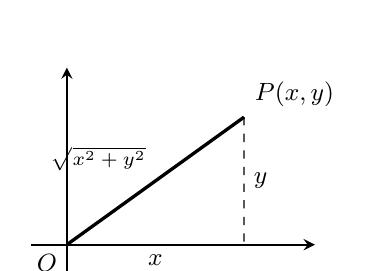
\begin{tikzpicture}[>=stealth, scale=0.9, font=\small]
  \draw[->, thick] (-0.5, 0) -- (3.5, 0);
  \draw[->, thick] (0, -0.5) -- (0, 2.5);
  \coordinate (O) at (0, 0);
  \coordinate (P) at (2.5, 1.8);
  \draw[very thick] (O) -- (P) node[above right] {$P(x, y)$};
  \draw[dashed] (P) -- (2.5, 0);
  \node[below left] at (O) {$O$};
  \node[below] at (1.25, 0) {$x$};
  \node[right] at (2.5, 0.9) {$y$};
  \node[above left] at (1.25, 0.9) {\scriptsize $\sqrt{x^2+y^2}$};
\end{tikzpicture}
\caption{平面點之原點距離}
\label{fig:b3-fig2-38}
\end{minipage}
\end{figure}

很自然，我們要問：對一般的三角形 $\triangle ABC$，\eqref{eq:b3-pythagoras} 式自是不一定成立，但我們是否能在 \eqref{eq:b3-pythagoras} 式插入一個校正項，使之對所有的三角形均成立？

為此，我們將考慮兩種意義的推廣，一為引入一個牽涉了餘弦的項來調整 \eqref{eq:b3-pythagoras} 式（此即所謂\textbf{餘弦定律}），一為引入一適當平行四邊形之另一對角線，來調整 \eqref{eq:b3-pythagoras} 式（此即所謂\textbf{平行四邊形定理}）.

\subsubsection*{甲、畢氏定理的推廣}

\begin{theorem}[第一廣義畢氏定理（餘弦定律）]
設一三角形三邊 $a, b, c$（$a, b, c$ 亦分別代表邊長）若 $a$ 與 $b$ 兩邊的夾角角度為 $\theta$，則
\begin{equation}
c^2 = a^2 + b^2 - 2ab\cos\theta \label{eq:b3-law-of-cosines}
\end{equation}
\end{theorem}

\begin{figure}[H]
\centering
\begin{minipage}{0.48\textwidth}
\centering
\begin{tikzpicture}[>=stealth, scale=1.0, font=\small]
  \coordinate (C) at (0, 0);
  \coordinate (B) at (3.5, 0);
  \coordinate (A) at (1.2, 2.2);
  \coordinate (D) at (1.2, 0);

  \draw[very thick] (C) -- (B) -- (A) -- cycle;
  \draw[dashed, thick] (A) -- (D);
  \draw (D) rectangle ++(0.2, 0.2);

  \node[left] at (C) {$C$};
  \node[right] at (B) {$B$};
  \node[above] at (A) {$A$};
  \node[below] at (D) {$D$};

  \node at (0.4, 0.25) {$\theta$};
  \node[left] at (0.6, 1.1) {$b$};
  \node[above right] at (2.35, 1.1) {$c$};
  \node[left] at (1.2, 1.1) {\scriptsize $b\sin\theta$};
  \node[below] at (0.6, 0) {\scriptsize $b\cos\theta$};
  \draw[<->] (0, -0.4) -- (3.5, -0.4) node[midway, below] {$a$};
  \node[below=0.6cm] at (1.75, 0) {（此時 $b\cos\theta > 0$）};
\end{tikzpicture}
\caption{銳角三角形餘弦定律證明}
\label{fig:b3-fig2-39-1}
\end{minipage}
\hfill
\begin{minipage}{0.48\textwidth}
\centering
\begin{tikzpicture}[>=stealth, scale=1.0, font=\small]
  \coordinate (C) at (1.5, 0);
  \coordinate (B) at (4.0, 0);
  \coordinate (A) at (0.5, 1.8);
  \coordinate (D) at (0.5, 0);

  \draw[very thick] (C) -- (B) -- (A) -- cycle;
  \draw[dashed, thick] (A) -- (D);
  \draw[dashed, thick] (D) -- (C);
  \draw (D) rectangle ++(0.2, 0.2);

  \node[below] at (C) {$C$};
  \node[right] at (B) {$B$};
  \node[above] at (A) {$A$};
  \node[below] at (D) {$D$};

  \node at (1.8, 0.25) {$\theta$};
  \node[above right] at (1.0, 0.9) {$b$};
  \node[above right] at (2.25, 0.9) {$c$};
  \node[left] at (0.5, 0.9) {\scriptsize $b\sin\theta$};
  \node[below] at (1.0, 0) {\scriptsize $-b\cos\theta$};
  \draw[<->] (1.5, -0.4) -- (4.0, -0.4) node[midway, below] {$a$};
  \node[below=0.6cm] at (2.25, 0) {（此時 $b\cos\theta < 0$）};
\end{tikzpicture}
\caption{鈍角三角形餘弦定律證明}
\label{fig:b3-fig2-39-2}
\end{minipage}
\end{figure}

\begin{proof}
在 $\triangle ABD$ 上，考慮畢氏定理，得
\begin{align*}
\overline{AD}^2 + \overline{DB}^2 &= \overline{AB}^2 \\
(b\sin\theta)^2 + (a - b\cos\theta)^2 &= c^2 \\
b^2 \sin^2\theta + a^2 - 2ab\cos\theta + b^2 \cos^2\theta &= c^2 \\
a^2 + b^2 - 2ab\cos\theta &= c^2 \quad\text{〔因 $\sin^2\theta + \cos^2\theta = 1$〕} \qedhere
\end{align*}
\end{proof}

\subsubsection*{作業 12}
\begin{enumerate}[label=\roman*), leftmargin=2.5em]
  \item 一個三角形若有一角為 $120^\circ$（或 $\frac{2\pi}{3}$），請給出一個三邊邊長間的關係.
  \item 設一鈍角三角形有一銳角為 $45^\circ$，而此銳角夾邊之比為 $\sqrt{2} : 1 + \sqrt{3}$，試問其他兩角為何？三邊之比為何？
\end{enumerate}

\begin{theorem}[第二廣義畢氏定理（平行四邊形定理）]
平行四邊形 $ACBD$ 兩對角線的平方和等於兩鄰邊平方和的兩倍，即圖 2-40 中
\begin{equation}
c^2 + d^2 = 2(a^2 + b^2) \label{eq:b3-parallelogram}
\end{equation}
\end{theorem}

\begin{figure}[H]
\centering
\begin{tikzpicture}[>=stealth, scale=1.0, font=\small]
  \coordinate (C) at (0, 0);
  \coordinate (B) at (3.5, 0);
  \coordinate (A) at (1.0, 1.8);
  \coordinate (D) at (4.5, 1.8);

  \draw[very thick] (C) -- (B) -- (D) -- (A) -- cycle;
  \draw[thick] (A) -- (B) node[midway, above] {$c$};
  \draw[dashed, thick] (C) -- (D) node[midway, above] {$d$};

  \node[left] at (C) {$C$};
  \node[right] at (B) {$B$};
  \node[above left] at (A) {$A$};
  \node[above right] at (D) {$D$};

  \node[below] at (1.75, 0) {$a$};
  \node[above] at (2.75, 1.8) {$a$};
  \node[left] at (0.5, 0.9) {$b$};
  \node[right] at (4.0, 0.9) {$b$};
  \node at (0.5, 0.2) {$\theta$};
\end{tikzpicture}
\caption{平行四邊形對角線定理}
\label{fig:b3-fig2-40}
\end{figure}

\begin{proof}
設 $\angle BCA = \theta$, $\angle DBC = \pi - \theta$.

則在 $\triangle BCA$ 及 $\triangle DBC$ 上分別使用餘弦定律，得
\begin{align*}
c^2 &= a^2 + b^2 - 2ab\cos\theta \\
d^2 &= a^2 + b^2 - 2ab\cos(\pi - \theta)
\end{align*}
但 $\cos(\pi - \theta) = -\cos\theta$，故上兩式相加得
\[ c^2 + d^2 = 2(a^2 + b^2) \qedhere \]
\end{proof}

作為餘弦定律的另一個應用，我們有

\begin{example}[圓的割線定理]
自圓外一點 $A$ 引一圓的割線交圓於 $B, C$ 兩點，另外引一切線 $AT$ 切圓於 $T$ 則
\begin{equation}
\overline{AB} \cdot \overline{AC} = \overline{AT}^2 \label{eq:b3-secant-theorem}
\end{equation}
\end{example}

\begin{figure}[H]
\centering
\begin{tikzpicture}[>=stealth, scale=1.0, font=\small]
  \coordinate (O) at (3, 0.8);
  \draw[thick] (O) circle (1.5cm);

  \coordinate (A) at (0, 0.6);
  % Tangent point T
  \coordinate (T) at (2.4, 2.18);
  \draw[thick] (A) -- (T) node[midway, above] {};
  \draw[thick] (O) -- (T) node[midway, right] {$r$};
  \node[above] at (T) {$T$};

  % Secant line ABC through circle
  \coordinate (B) at (1.8, 0.4);
  \coordinate (C) at (4.3, 0.1);
  \draw[thick] (A) -- (C);
  \draw[dashed] (O) -- (A) node[midway, above] {$a$};
  \draw[dashed] (O) -- (B) node[midway, below] {$r$};
  \draw[dashed] (O) -- (C) node[midway, right] {$r$};

  \node[left] at (A) {$A$};
  \node[below] at (B) {$B$};
  \node[right] at (C) {$C$};
  \node[right] at (O) {$O$};

  \node[below] at (0.9, 0.5) {$b$};
  \node[below] at (3.0, 0.25) {$u$};
  \node at (0.8, 0.7) {$\theta$};
\end{tikzpicture}
\caption{圓的割線定理餘弦證明}
\label{fig:b3-fig2-41}
\end{figure}

\begin{proof}
設圓心為 $O$，半徑為 $r$，而 $\angle OAB = \angle OAC = \theta$. 則在 $\triangle OAB$ 及 $\triangle OAC$ 上分別使用餘弦定律，得
\begin{align}
r^2 &= a^2 + b^2 - 2ab\cos\theta \label{eq:b3-secant-1} \\
r^2 &= a^2 + (b+u)^2 - 2a(b+u)\cos\theta \label{eq:b3-secant-2}
\end{align}
其中 $\overline{AB} = b, \overline{BC} = u, \overline{OA} = a$.

今欲從 \eqref{eq:b3-secant-1}, \eqref{eq:b3-secant-2} 兩式中消去 $\cos\theta$，求得 $b, u$ 與 $r, a$ 的關係.（注意：$\cos\theta \ne 0$，因 $A$ 在圓外）.

\eqref{eq:b3-secant-2} 減 \eqref{eq:b3-secant-1} 得：
\begin{align*}
2bu + u^2 - 2au\cos\theta &= 0 \\
2b + u - 2a\cos\theta &= 0 \quad\text{〔因 $u=0$ 時，\eqref{eq:b3-secant-theorem} 式已自動成立，不需證明〕}
\end{align*}
但由上式：$2a\cos\theta = 2b + u$. 代入 \eqref{eq:b3-secant-1}：
\[ r^2 = a^2 + b^2 - b(2b + u) \]
即
\[ b(b+u) = a^2 - r^2 \]
亦即
\[ \overline{AB} \cdot \overline{AC} = \overline{AT}^2 \quad\text{〔在右端使用畢氏定理〕} \qedhere \]
\end{proof}

\textbf{另證}：本定理採用平面幾何單純的相似形原理，立可證得：
\begin{align*}
\text{因}\quad \angle ATB &= \angle ACT \quad\text{〔為什麼？〕} \\
\text{故}\quad \triangle ATB &\sim \triangle ACT \\
\text{而得}\quad \frac{\overline{AT}}{\overline{AB}} &= \frac{\overline{AC}}{\overline{AT}} \\
\text{即}\quad \overline{AB} \cdot \overline{AC} &= \overline{AT}^2 \qedhere
\end{align*}

\textbf{分析}\quad 上述第一證法表面上看似乎稍嫌繁複，但它的道理實際上只是「在 $\triangle OAB$ 與 $\triangle OAC$ 上分別施用餘弦定律」這一想法，以後便是單純的代數運算. 這樣做法有什麼好處？態度上這種做法是在尋求未知，而不是在證明已知. 因為通過觀察我們看出使用兩次餘弦定律必得到兩個 $r, u, a, b$ 與 $\cos\theta$ 五個量間的關係式，只要這兩個式子互相獨立，則 $\cos\theta$ 可望消去，而得到 $r, u, a, b$ 間的一個關係式. 這個關係式經單純的運算後，只是湊巧發覺它原來是已知的割線定理，這種主動的與系統的過程是數學發展中重要的方法.

\subsubsection*{乙、三角形之面積與邊長}

餘弦定律也幫我們找出一個三角形面積與其邊長、周長的關係.

\begin{theorem}[餘弦定律的應用：三角形面積與邊長]
設一三角形 $\triangle ABC$ 三邊邊長分別為 $a, b, c$，$\Delta$ 表其面積，$s$ 表其周長之半，即
\[ s = \frac{1}{2}(a+b+c) \]
則
\begin{equation}
\Delta^2 = s(s-a)(s-b)(s-c) \label{eq:b3-heron}
\end{equation}
\end{theorem}

\begin{figure}[H]
\centering
\begin{tikzpicture}[>=stealth, scale=1.0, font=\small]
  \coordinate (A) at (0, 0);
  \coordinate (B) at (4, 0);
  \coordinate (C) at (2.4, 2.0);
  \coordinate (D) at (2.4, 0);

  \draw[very thick] (A) -- (B) -- (C) -- cycle;
  \draw[dashed, thick] (C) -- (D);
  \draw (D) rectangle ++(-0.2, 0.2);

  \node[left] at (A) {$A$};
  \node[right] at (B) {$B$};
  \node[above] at (C) {$C$};
  \node[below] at (2.4, 0) {};

  \node[above left] at (1.2, 1.0) {$b$};
  \node[above right] at (3.2, 1.0) {$a$};
  \node[below] at (2.0, 0) {$c$};
\end{tikzpicture}
\caption{三角形邊長與面積}
\label{fig:b3-fig2-42}
\end{figure}

\begin{proof}
$\triangle ABC$ 之底為 $c$，高為 $b\sin A$，其面積
\begin{align*}
\Delta &= \frac{1}{2}bc\sin A \\
\Delta^2 &= \frac{1}{4}b^2 c^2 \sin^2 A = \frac{1}{4}b^2 c^2(1 - \cos^2 A) \\
&= \frac{1}{4}b^2 c^2\left\{1 - \left(\frac{b^2 + c^2 - a^2}{2bc}\right)^2\right\} \\
&= \frac{1}{4}b^2 c^2\left[1 + \frac{b^2 + c^2 - a^2}{2bc}\right]\left[1 - \frac{b^2 + c^2 - a^2}{2bc}\right] \\
&= \frac{1}{16}\left[2bc + b^2 + c^2 - a^2\right]\left[2bc - b^2 - c^2 + a^2\right] \\
&= \frac{1}{16}\left[(b+c)^2 - a^2\right]\left[a^2 - (b-c)^2\right] \\
&= \frac{1}{16}(a+b+c)(-a+b+c)(a-b+c)(a+b-c) \\
&= s(s-a)(s-b)(s-c) \qedhere
\end{align*}
\end{proof}

下面的正弦定律，在測量上時常用到：

\begin{theorem}[正弦定律]
三角形各內角角度之正弦與其對角邊長之比一樣，意即：在 $\triangle ABC$ 中，
\begin{equation}
\frac{\sin A}{a} = \frac{\sin B}{b} = \frac{\sin C}{c} \label{eq:b3-law-of-sines}
\end{equation}
\end{theorem}

\begin{figure}[H]
\centering
\begin{minipage}{0.48\textwidth}
\centering
\begin{tikzpicture}[>=stealth, scale=0.95, font=\small]
  \coordinate (A) at (0, 0);
  \coordinate (B) at (3.5, 0);
  \coordinate (C) at (1.8, 2.2);
  \coordinate (D) at (1.8, 0);

  \draw[very thick] (A) -- (B) -- (C) -- cycle;
  \draw[dashed, thick] (C) -- (D);
  \draw (D) rectangle ++(0.2, 0.2);

  \node[left] at (A) {$A$};
  \node[right] at (B) {$B$};
  \node[above] at (C) {$C$};

  \node[left] at (0.9, 1.1) {$b$};
  \node[right] at (2.65, 1.1) {$a$};
  \node[below] at (1.75, 0) {$c$};
  \node[left] at (1.8, 1.0) {$h$};
\end{tikzpicture}
\caption{銳角三角形正弦定律}
\label{fig:b3-fig2-43-1}
\end{minipage}
\hfill
\begin{minipage}{0.48\textwidth}
\centering
\begin{tikzpicture}[>=stealth, scale=0.95, font=\small]
  \coordinate (A) at (1.2, 0);
  \coordinate (B) at (3.5, 0);
  \coordinate (C) at (0.4, 2.0);
  \coordinate (D) at (0.4, 0);

  \draw[very thick] (A) -- (B) -- (C) -- cycle;
  \draw[dashed, thick] (C) -- (D);
  \draw[dashed, thick] (D) -- (A);
  \draw (D) rectangle ++(0.2, 0.2);

  \node[below] at (A) {$A$};
  \node[right] at (B) {$B$};
  \node[above] at (C) {$C$};

  \node[above right] at (0.8, 1.0) {$b$};
  \node[above right] at (2.0, 1.0) {$a$};
  \node[below] at (2.35, 0) {$c$};
  \node[left] at (0.4, 1.0) {$h$};
\end{tikzpicture}
\caption{鈍角三角形正弦定律}
\label{fig:b3-fig2-43-2}
\end{minipage}
\end{figure}

\begin{proof}
自 $C$ 作 $AB$ 垂線，表此垂線長為 $h$，則根據正弦定義
\[ b\sin A = h = a\sin B \]
故
\[ \frac{\sin A}{a} = \frac{\sin B}{b} \]
同理
\[ \frac{\sin B}{b} = \frac{\sin C}{c} \quad\text{故得證.} \qedhere \]
\end{proof}

\begin{example}
設三角形三邊分別為 $a = 255.18$, $b = 290.87$, $c = 419.25$，試求 $\Delta$ 之面積.
\end{example}

\begin{proof}[解]
由定理 3 得 $\Delta = \sqrt{s(s-a)(s-b)(s-c)}$，把各值代入即可求算得.

但是，以上數字計算相當麻煩. 為簡化起見，可以應用對數原則：$\log xy = \log x + \log y$（第二冊第四章）來計算. 此地取以 10 為底的對數，各對數值查表（附錄三）可得.
\begin{align*}
a &= 255.18 & s-a &= 227.47 & \log_{10}(s-a) &= 2.35692 \\
b &= 290.87 & s-b &= 191.78 & \log_{10}(s-b) &= 2.28280 \\
c &= 419.25 & s-c &= 63.40  & \log_{10}(s-c) &= 1.80209 \\
2s &= 965.30 & s &= 482.65 & \log s &= 2.68364 \\
s &= 482.65 & & & 2\log\Delta &= 9.12545 \\
& & & & \log\Delta &= 4.56272 \\
& & & & \therefore\quad \Delta &= 36536 \qedhere
\end{align*}
\end{proof}

\begin{example}
試證：四邊形面積等於二對角線與對角線夾角正弦乘積之半.
\end{example}

\begin{figure}[H]
\centering
\begin{tikzpicture}[>=stealth, scale=0.9, font=\small]
  \coordinate (O) at (0, 0);
  \coordinate (A) at (2.2, 0.4);
  \coordinate (C) at (-2.0, -0.4);
  \coordinate (D) at (-0.3, 1.2);
  \coordinate (B) at (0.5, -1.4);

  \draw[very thick] (A) -- (D) -- (C) -- (B) -- cycle;
  \draw[thick] (A) -- (C);
  \draw[thick] (B) -- (D);

  \node[right] at (A) {$A$};
  \node[left] at (C) {$C$};
  \node[above] at (D) {$D$};
  \node[below] at (B) {$B$};
  \node[below left] at (O) {$O$};
  \node at (0.3, 0.2) {$\theta$};
\end{tikzpicture}
\caption{任意四邊形對角線面積公式}
\label{fig:b3-fig2-44}
\end{figure}

\begin{proof}
設對角線 $AC$ 與 $BD$ 交於 $O$，夾角為 $\theta$. 則
\begin{align*}
ABCD\text{ 之面積} &= \triangle ABC + \triangle ADC \\
&= \frac{1}{2}\overline{OB}\sin\theta \cdot \overline{AC} + \frac{1}{2}\overline{OD}\sin\theta \cdot \overline{AC} \\
&= \frac{1}{2}\overline{BD}\cdot \overline{AC}\cdot \sin\theta \qedhere
\end{align*}
\end{proof}

\subsection*{習題 2-4}
\label{ex:b3-ch2-p59-2-4}

\begin{enumerate}[label=\arabic*., leftmargin=2em]
  \item $\triangle ABC$ 中已知 $a = \frac{\sqrt{3}+1}{2\sqrt{2}}$, $b = \frac{\sqrt{3}-1}{2\sqrt{2}}$, $c = \frac{\sqrt{3}}{2}$. 求 $\angle A, \angle B, \angle C$.〔提示：$\cos 15^\circ = \frac{\sqrt{6}+\sqrt{2}}{4}$〕
  \item 在 $\triangle ABC$ 中，已知 $\angle A = 60^\circ$, $b = (2+\sqrt{3})c$. 求 $\angle B$ 及 $\angle C$.
  \item 在 $\triangle ABC$ 中，已知三邊長為 $3, 5, 6$.
  \begin{enumerate}[label=(\roman*), leftmargin=2.5em]
    \item 求 $\triangle ABC$ 的面積
    \item 求 $\triangle ABC$ 內切圓的半徑.
  \end{enumerate}
  〔提示：$\Delta = \triangle ABC\text{ 面積} = \triangle AOB, \triangle BOC, \triangle COA\text{ 諸面積和，以 } r, a, b, c\text{ 表 }\Delta$〕
  \begin{flushright}
  \begin{tikzpicture}[>=stealth, scale=0.85, baseline=(current bounding box.center)]
    \coordinate (B) at (0, 0);
    \coordinate (C) at (3.5, 0);
    \coordinate (A) at (2.2, 2.2);
    \draw[thick] (B) -- (C) -- (A) -- cycle;
    \coordinate (O) at (2.0, 0.7);
    \draw (O) circle (0.7cm);
    \draw[dashed] (O) -- (A);
    \draw[dashed] (O) -- (B);
    \draw[dashed] (O) -- (C);
    \draw[->] (O) -- ++(0, -0.7) node[midway, right] {$r$};
    \node[left] at (B) {$B$};
    \node[right] at (C) {$C$};
    \node[above] at (A) {$A$};
    \node[above left] at (O) {$O$};
  \end{tikzpicture}
  \end{flushright}
\end{enumerate}

\subsection{\texorpdfstring{$\ddagger$ }{‡ }三角測量}
\label{subsec:b3-2-5}

在國中我們學過一些簡易的三角形測量，這些測量距離或高度的理論基礎是：把地面上的山川形勢這些大的圖形縮小到紙上作業，根據相似形原理，原來大圖形上面諸高度或距離之間的比例並不因縮小到紙上而變. 另一方面，這些比例（例如直角三角形的直角邊與斜邊之比，便是正弦、餘弦）可在紙上量出（量出來的結果我們已系統化，編成三角函數表），故只要地面上的大圖形裏頭有一已知的高度或距離，則可根據那已知的比例算出所求的高度或距離. 注意這已知的高度或距離是不能沒有的，只知道圖形上各邊比例而不知它的放大率終歸是紙上談兵. 現場測量得的資料是必須的.

先回想一下國中所唸過的三角測量，提出進一步測量的問題，然後再利用我們所學的一般角的三角函數，餘弦定律，正弦定律逐一解決.

\textbf{第一類型}：

\begin{figure}[H]
\centering
\begin{tikzpicture}[>=stealth, scale=0.9, font=\small]
  \coordinate (A) at (0, 0);
  \coordinate (B) at (0, 2.5);
  \coordinate (C) at (4, 2.5);

  % Watchtowers & Ship
  \draw[very thick] (A) -- (B) node[midway, left] {$b$};
  \draw[thick] (B) -- (C);
  \draw[thick] (A) -- (C) node[midway, below] {$d = {?}$};

  % Waves on sea
  \foreach \y in {0.2, 0.4,...,2.3} {
    \draw[gray!50] (0.2, \y) -- (1.5, \y);
  }

  \node[left] at (A) {$A$};
  \node[left] at (B) {$B$};
  \node[above right] at (C) {$C$ (船)};

  \node at (0.3, 0.3) {$\alpha$};
  \node at (0.3, 2.2) {$\beta$};
  \node at (3.5, 2.3) {$\gamma$};
\end{tikzpicture}
\caption{兩瞭望臺測海中船隻距離}
\label{fig:b3-fig2-46}
\end{figure}

設 $A, B$ 處有兩瞭望臺，兩臺之間距離為 $b$，今發現海上有船 $C$. 欲求 $AC$ 距離 $d$（或 $BC$ 距離）.

回想國中的算法，其實就是我們剛學的正弦定律的證明. 正弦定律現在儘可以直接使用，不須每一次都要重導.

「分別在瞭望臺 $A, B$ 處測量 $\alpha$ 及 $\beta$ 兩角，於是亦可得知
\[ \gamma = \angle ACB = \pi - \alpha - \beta \]
根據正弦定律
\[ \frac{\sin\beta}{d} = \frac{\sin\gamma}{b} \]
故 $d = \frac{b\sin\beta}{\sin\gamma}$ 立可求得」

但一般時候，那船 $C$ 的位置不一定恰好會使 $\triangle ABC$ 構成一銳角三角形.

很可能狀況是這樣的：

\begin{figure}[H]
\centering
\begin{tikzpicture}[>=stealth, scale=0.9, font=\small]
  \coordinate (A) at (0, 0);
  \coordinate (B) at (0.5, 1.5);
  \coordinate (C) at (3.5, 3.0);

  \draw[very thick] (A) -- (B) node[midway, left] {$b$};
  \draw[thick] (B) -- (C);
  \draw[thick] (A) -- (C);

  \node[left] at (A) {$A$};
  \node[left] at (B) {$B$};
  \node[above right] at (C) {$C$ (船)};

  \node at (0.3, 0.4) {$\alpha$};
  \node at (0.7, 1.4) {$\beta$};
\end{tikzpicture}
\caption{鈍角觀測情境}
\label{fig:b3-fig2-47}
\end{figure}

\textbf{問題 A}\quad “當 $\beta$ 為鈍角，問瞭望臺 $A$ 與船 $C$ 相隔多遠？”

這種狀況因國中的教材只提銳角三角函數，因此就難以使用. 現在既然已引入了鈍角三角函數且知正弦定律仍然成立，故剛剛敘述過的方法就可以用了.

\phantomsection\label{note:b3-ch2-p60-ex12-data}%
\begin{example}
若 $\alpha = 45^\circ$, $\beta = 105^\circ$, $b = 1000\sqrt{6}$ 公尺\footnote{【校訂註】原書例 12 題幹印作「$b = 1000\sqrt{6}$ 公尺」，解文中計算代入數值為 $100\sqrt{6}$ 公尺，算得結果 $467.5$ 公尺，題幹數值多植一零。正文照原印字樣錄入。}，則船 $C$ 與瞭望台 $A$ 相距多遠？
\end{example}

\begin{proof}[解]
$\gamma = \angle ACB = 180^\circ - \alpha - \beta = 30^\circ$.

由正弦定律：$\frac{\sin\beta}{\overline{AC}} = \frac{\sin\gamma}{b}$，並查正弦函數表
\[ \overline{AC} = b\frac{\sin 105^\circ}{\sin 30^\circ} = 100\sqrt{6}\frac{0.9659}{\frac{1}{2}} \doteq 467.5\text{ 公尺.} \qedhere \]
\end{proof}

\textbf{第二類型}：已知山上一塔之高，欲求山高.

\begin{figure}[H]
\centering
\begin{tikzpicture}[>=stealth, scale=0.9, font=\small]
  % Mountain shape
  \draw[thick] (-1, 0) to[out=40, in=180] (2.5, 2.5) to[out=0, in=140] (4.5, 0);
  % Tower B1 B2
  \coordinate (B1) at (2.5, 2.5);
  \coordinate (B2) at (2.5, 3.2);
  \coordinate (C) at (2.5, 0);
  \draw[very thick] (B1) -- (B2);
  \draw[dashed] (B1) -- (C);

  % Observation point A
  \coordinate (A) at (-1.5, 0);
  \draw[thick] (A) -- (C);
  \draw[thick] (A) -- (B1);
  \draw[thick] (A) -- (B2);

  \node[left] at (A) {$A$};
  \node[below] at (C) {$C$};
  \node[right] at (B1) {$B_1$};
  \node[right] at (B2) {$B_2$};

  \node at (-0.5, 0.2) {$\alpha$};
  \node at (-0.5, 0.5) {$\beta$};
\end{tikzpicture}
\caption{測量山上塔高與山高}
\label{fig:b3-fig2-48}
\end{figure}

我們的方法是在平地 $A$ 點測得仰角 $\alpha$ 及 $\beta$，接著查表得知 $\tan\alpha, \tan\beta$，然後利用所知塔高 $\overline{B_1 B_2}$，由下式
\[ \tan\alpha - \tan\beta = \frac{\overline{CB_2}}{\overline{AC}} - \frac{\overline{CB_1}}{\overline{AC}} = \frac{\overline{B_1 B_2}}{\overline{AC}} \]
算出 $\overline{AC}$，則山高 $\overline{CB_1} = \overline{AC}\tan\beta$ 即可求出.

（注意這時候塔高 $\overline{B_1 B_2}$ 是一已知邊，其餘利用三角函數求測可得）.

\phantomsection\label{note:b3-ch2-p61-ex13-sir}%
\begin{example}
設一塔，高 125 公尺，立在河邊山岩上. 從塔頂俯望對岸的俯角為 $28^\circ 40'$，而從塔腳俯望對岸同點俯角為 $18^\circ 20'$ 試求山岩高及河寬.
\end{example}

\begin{figure}[H]
\centering
\begin{tikzpicture}[>=stealth, scale=0.9, font=\small]
  \coordinate (D) at (4, 0);
  \coordinate (B) at (4, 1.2);
  \coordinate (C) at (4, 2.2);
  \coordinate (A) at (0, 0);

  \draw[thick] (A) -- (D) node[midway, below] {};
  \draw[very thick] (B) -- (C) node[midway, right] {$a$};
  \draw[thick] (D) -- (B);
  \draw[thick] (A) -- (B) node[midway, below right] {$c$};
  \draw[thick] (A) -- (C) node[midway, above] {$b$};

  \node[left] at (A) {$A$};
  \node[right] at (D) {$D$};
  \node[right] at (B) {$B$};
  \node[right] at (C) {$C$};

  % Depression angles
  \draw[dashed] (C) -- ++(-2, 0);
  \draw[dashed] (B) -- ++(-2, 0);
  \node[left] at (3.2, 2.2) {\scriptsize $28^\circ 40'$};
  \node[left] at (3.2, 1.2) {\scriptsize $18^\circ 20'$};
  \node at (1.2, 0.2) {$\gamma$};
\end{tikzpicture}
\caption{懸崖塔頂俯角測量河寬}
\label{fig:b3-fig2-49}
\end{figure}

\begin{proof}[解]
在圖 2-49 $CB$ 表示塔高，$BD$ 表山岩，$A$ 表河對岸所取的位置，此題為第二類型，但可以只用正弦，餘弦來做，因
\[ \angle\gamma = 28^\circ 40' - 18^\circ 20' = 10^\circ 20' \]
由正弦定律得\footnote{【校訂註】原書排印為「$a \text{ sir}(\frac{\pi}{2} - 28^\circ 40')$」，英文正弦函數記號「$\sin$」誤植為「sir」。正文照原刊字樣錄入。}
\[ c = \frac{a\sin\left(\frac{\pi}{2}-28^\circ 40'\right)}{\sin(10^\circ 20')} = \frac{125(0.8774)}{0.1794} \doteq 611. \]
故
\begin{align*}
\overline{BD} &= c\sin 18^\circ 20' = 611(0.3145) = 192\text{ 公尺} \\
\overline{AD} &= c\cos 18^\circ 20' = 611(0.9492) = 580\text{ 公尺} \qedhere
\end{align*}
\end{proof}

現在我們提出一個較複雜的問題：

\textbf{問題 B}\quad “如果我們不知塔高多少，有無辦法求測山高？”

也就是這時，我們沒有現成的已知邊，須就實際情形作出一已知邊.（關鍵在作一已知邊後利用正弦定律）

\textbf{方法}\quad 設 $B$ 為山峯，在地面上取 $A_1$ 與 $A_2$ 兩點，分別測出角度 $\gamma$, $\alpha$ 及 $\overline{A_1 A_2} = b$（這 $A_1 A_2$ 便是作出來的已知邊）又在 $A_1$ 點可測得仰角 $\theta$.

\begin{figure}[H]
\centering
\begin{tikzpicture}[>=stealth, scale=0.9, font=\small]
  % 3D hill
  \coordinate (C) at (2.5, 0);
  \coordinate (B) at (2.5, 2.8);
  \coordinate (A1) at (1.0, -1.0);
  \coordinate (A2) at (-1.0, 0);

  \draw[very thick] (C) -- (B) node[midway, right] {$h$};
  \draw[thick] (A1) -- (B);
  \draw[thick] (A2) -- (B);
  \draw[thick] (A1) -- (A2) node[midway, below left] {$b$};
  \draw[dashed] (A1) -- (C) node[midway, below right] {$d$};
  \draw[dashed] (A2) -- (C);

  \node[below] at (C) {$C$};
  \node[above] at (B) {$B$};
  \node[below] at (A1) {$A_1$};
  \node[left] at (A2) {$A_2$};

  \node at (0.9, -0.6) {$\theta$};
  \node at (-0.4, 0.1) {$\alpha$};
  \node at (0.8, -0.3) {$\gamma$};
\end{tikzpicture}
\caption{立體三角測量山高}
\label{fig:b3-fig2-50}
\end{figure}

今 $\beta = \pi - (\alpha + \gamma)$ 可以求得，而由正弦定律得 $\frac{\sin\beta}{b} = \frac{\sin\alpha}{a}$，故
\[ a = \frac{b\sin\alpha}{\sin\beta} \text{ 成爲已知} \]
所求 $h = a\sin\theta = \frac{ab\sin\alpha\sin\theta}{\sin\beta}$ 便可求得.

\textbf{注意}\quad 地形上許可時，可取 $A_1, A_2$ 使 $A_1, A_2, C$ 三點共線. 這是平常的作法. 但實際上要使測量準確，須要求兩觀測點 $A_1$ 與 $A_2$ 之間距相當大. 而時常又無法尋得足夠寬廣而平坦的地面容許所選的觀測點 $A_1, A_2$ 與 $C$ 點共線. 以下舉一能選得 $A_1, A_2$ 使 $A_1, A_2, C$ 共線之例.

\begin{example}
某人測得一山峯之仰角為 $30^\circ$，當他向山腳前進 $\frac{1}{2}$ 公里再測量，得山峯之仰角增大切為 $45^\circ$，試求山高.
\end{example}

\begin{figure}[H]
\centering
\begin{tikzpicture}[>=stealth, scale=0.9, font=\small]
  \coordinate (A1) at (0, 0);
  \coordinate (A2) at (2.0, 0);
  \coordinate (C) at (4.0, 0);
  \coordinate (B) at (4.0, 2.0);

  \draw[thick] (A1) -- (C);
  \draw[very thick] (C) -- (B) node[midway, right] {$h = {?}$};
  \draw[thick] (A1) -- (B);
  \draw[thick] (A2) -- (B);

  \node[below] at (A1) {$A_1$};
  \node[below] at (A2) {$A_2$};
  \node[below] at (C) {$C$};
  \node[above] at (B) {$B$};

  \node at (0.8, 0.25) {$30^\circ$};
  \node at (2.6, 0.3) {$45^\circ$};
  \node at (2.2, 0.6) {$\alpha$};
  \node at (3.5, 1.6) {$\beta$};

  \draw[<->] (0, -0.4) -- (2.0, -0.4) node[midway, below] {$\frac{1}{2}$公里};
\end{tikzpicture}
\caption{共線兩點推進測量山高}
\label{fig:b3-fig2-51}
\end{figure}

\begin{proof}[解]
設 $A_1, A_2$ 為觀測點，$B$ 為頂峯，$C$ 為山腳，則由正弦定律得
\[ \frac{\sin\beta}{\overline{A_1 A_2}} = \frac{\sin 30^\circ}{\overline{A_2 B}} \]
\[ \therefore\quad \overline{A_2 B} = 1/2 \cdot \frac{\sin 30^\circ}{\sin 15^\circ} \doteq \frac{1}{2.449 - 1.414} = \frac{1}{1.035} \]
故山高
\[ h = \overline{BC} = \overline{A_2 B}\sin 45^\circ = \frac{1}{1.035} \times \frac{1}{\sqrt{2}} \doteq 0.683\text{ 公里} = 683\text{ 公尺.} \qedhere \]
\end{proof}

以上這兩種類型的題目，關鍵都在於正弦定律，正弦定律敘述兩個邊，兩個角間的關係. 平常角是比較容易測量，若有一已知邊，則可求另一未知邊. 因此正弦定律一般時候是相當夠用，但在一些視線不佳的情況下，要測到兩角就有點困難，此時餘弦定律便可考慮使用，因此只用到一個角.

\textbf{第三類型}：設有一湖欲測對岸兩點 $A$ 與 $B$ 間的距離.

假設由於地理限制，所選觀測點 $C$ 到 $A$ 與 $B$ 點連成兩線間的夾角 $\theta$ 不能正好是直角，此時畢氏定理不能施用.

如果從 $A$ 點可看得見 $B$ 點時，我們只要測出 $a, \theta$ 及 $\angle CAB$，則可用正弦定律求出 $c$.

但假設湖上視線不佳，測不出 $\angle CAB$ 則改用餘弦定律可立即求得 $c$：
\[ c^2 = a^2 + b^2 - 2ab\cos\theta \]

\begin{figure}[H]
\centering
\begin{tikzpicture}[>=stealth, scale=0.9, font=\small]
  \coordinate (C) at (0, 0);
  \coordinate (A) at (3.5, 1.2);
  \coordinate (B) at (3.0, -1.0);

  % Lake hatched area
  \fill[pattern=north east lines] (2.8, -1.2) to[out=40, in=-120] (3.8, 1.4) to[out=160, in=20] (2.8, -1.2);
  \draw[thick] (A) -- (B) node[midway, right] {$c$};
  \draw[thick] (C) -- (A) node[midway, above] {$b$};
  \draw[thick] (C) -- (B) node[midway, below] {$a$};

  \node[left] at (C) {$C$};
  \node[above] at (A) {$A$};
  \node[below] at (B) {$B$};
  \node at (0.6, 0.1) {$\theta$};
\end{tikzpicture}
\caption{隔湖測量不可達距離}
\label{fig:b3-fig2-52}
\end{figure}

\begin{example}
某人在岸邊小土墩上看一漁船在海岸附近慢行. 假設他已知土墩高出水面 20 公尺，但他受困在土墩上，不能走動. 現在他想知道船速如何，該如何測量？（假設船等速前進）
\end{example}

\begin{figure}[H]
\centering
\begin{tikzpicture}[>=stealth, scale=0.9, font=\small]
  \coordinate (B) at (2.5, 0);
  \coordinate (A) at (2.5, 1.8);
  \coordinate (C) at (-1.5, 0.8);
  \coordinate (D) at (0.2, -0.8);

  \draw[very thick] (B) -- (A) node[midway, right] {20公尺};
  \draw[thick] (A) -- (C);
  \draw[thick] (A) -- (D);
  \draw[dashed, thick] (C) -- (D);

  \node[right] at (A) {$A$};
  \node[right] at (B) {$B$};
  \node[above left] at (C) {$C$ (初)};
  \node[below] at (D) {$D$ (終)};

  % Angles
  \node at (1.5, 1.6) {\scriptsize $30^\circ$};
  \node at (1.7, 1.2) {\scriptsize $45^\circ$};
  \node at (-0.8, 0.7) {\scriptsize $30^\circ$};
  \node at (0.8, -0.6) {\scriptsize $45^\circ$};
\end{tikzpicture}
\caption{岸上高處觀測運動船速}
\label{fig:b3-fig2-53}
\end{figure}

\begin{proof}[解]
第一步先俯身測得觀測點對船之俯角，設為 $30^\circ$. 以 $C$ 表示此時船之位置，$A$ 為觀測點，則
\[ \overline{AC} = \frac{\overline{AB}}{\cos 60^\circ} = 40\text{ 公尺} \]
此時還應標出 $\vec{AC}$ 的方位.

過五分鐘（適當的時間）後，設船行至 $D$，再測得俯角為 $45^\circ$. 則船與墩頂距離變成
\[ \overline{AD} = \frac{\overline{AB}}{\cos 45^\circ} = 20\sqrt{2}\text{ 公尺} \]
此時亦標出 $\vec{AD}$ 的方位，並測出 $\angle CAD$ 的大小. 設為 $45^\circ$. 則由餘弦定律得船在五分鐘所行距離
\[ \overline{CD} = \sqrt{\overline{AD}^2 + \overline{AC}^2 - 2\overline{AD}\cdot\overline{AC}\cos 45^\circ} = 20\sqrt{2}\text{ 公尺} \]
故 船速 $= 20\sqrt{2}\text{ 公尺} / 5\text{ 分鐘} \doteq 5.656\text{ 公尺每秒.}$ \qedhere
\end{proof}

\subsubsection*{作業 13}
某人於一樓房，欲測對面一建築物之高度，假設這人無法離開此樓（但可在樓中上下），問他將如何測量？

\subsubsection*{作業 14}
設有甲乙兩山，一人從平地 $A$ 點爬上乙山，想藉此求得甲山高度：

\begin{figure}[H]
\centering
\begin{tikzpicture}[>=stealth, scale=0.9, font=\small]
  % Two mountains
  \coordinate (A) at (0, 0);
  \coordinate (P) at (2.0, 0);
  \coordinate (N) at (2.0, 0.8);
  \coordinate (M) at (3.5, 3.0);
  \coordinate (Q) at (3.5, 1.8);
  \coordinate (R) at (3.5, 1.2);
  \coordinate (Z) at (3.5, 0);

  \draw[thick] (A) -- (N) node[midway, above left] {};
  \draw[thick] (N) -- (M);
  \draw[dashed] (A) -- (P);
  \draw[dashed] (M) -- (Z);

  \node[left] at (A) {$A$};
  \node[above] at (M) {$M$};
  \node[right] at (N) {$N$};
  \node[below] at (P) {$P$};
  \node[below] at (Z) {乙};

  \node at (0.8, 0.15) {\scriptsize $30^\circ$};
  \node at (1.8, 1.4) {\scriptsize $60^\circ$};
\end{tikzpicture}
\caption{雙山高低聯測}
\label{fig:b3-fig2-54}
\end{figure}

設 $M, N$ 分別為甲乙兩山山頂，此人從 $A$ 沿直線斜坡 $AN$ 爬上乙山，$\overline{AN} = 800$ 公尺.

設一開始測得 $\angle MAN = 15^\circ$，又知 $AN$ 之傾斜角為 $30^\circ$. 此人爬到乙山山頂 $N$ 時又測得對 $M$ 點仰角為 $60^\circ$，且 $\angle ANM = 120^\circ$，問甲山山高多少？

\subsubsection*{作業 15}
一船向東 $37^\circ$ 南航行，速度為 30 浬/時，於上午 9 時測得，測得一島之方向為東 $53^\circ$ 北，到中午 12 時再測，得該島之方向在船之北 $23^\circ$ 西，試求當時（中午時）船與島距離.

\phantomsection\label{note:b3-ch2-p66-homework16-deg}%
\subsubsection*{作業 16}
設有一湖，欲測湖岸兩點 $CD$ 長，但湖岸築有鐵絲網不能靠近，在鐵絲網外取 $A, B$，兩點間距離為 30 公尺，分別自 $A, B$ 可看到其餘三點 $C, D, B$ 或 $C, D, A$. 因而測得（見圖）
\begin{align*}
\angle CAB &= 120\footnote{【校訂註】原書印作「$\angle CAB = 120$」，漏印度數符號「$^\circ$」，實為 $120^\circ$。正文照原刊樣式錄入。}, & \angle CBA &= 35^\circ \\
\angle DAB &= 45^\circ, & \angle DBA &= 75^\circ
\end{align*}
求 $\overline{CD}$ 長.

\begin{figure}[H]
\centering
\begin{minipage}{0.45\textwidth}
\centering
\begin{tikzpicture}[>=stealth, scale=0.85, font=\small]
  \coordinate (O) at (0, 0);
  \draw[->, thick] (O) -- (0, 2) node[above] {$N$};
  \draw[->, thick] (O) -- (2, 0) node[right] {$E$};
  \coordinate (Ship) at (-0.8, 0.6);
  \draw[->, thick] (O) -- (40:2) node[above right] {島};
  \draw[->, very thick] (O) -- (-37:2) node[below right] {30浬/時};
  \node at (0.5, 0.3) {\scriptsize $53^\circ$};
  \node at (0.5, -0.2) {\scriptsize $37^\circ$};
\end{tikzpicture}
\caption{航海航向與方位測量}
\label{fig:b3-fig2-55}
\end{minipage}
\hfill
\begin{minipage}{0.5\textwidth}
\centering
\begin{tikzpicture}[>=stealth, scale=0.85, font=\small]
  \coordinate (A) at (0, 0);
  \coordinate (B) at (3, 0);
  \coordinate (C) at (0.8, 2.2);
  \coordinate (D) at (3.5, 2.5);

  \draw[very thick] (A) -- (B) node[midway, below] {$a$};
  \draw[thick] (A) -- (C);
  \draw[thick] (A) -- (D);
  \draw[thick] (B) -- (C);
  \draw[thick] (B) -- (D);
  \draw[thick] (C) -- (D);

  % Fence line
  \draw[decorate, decoration={zigzag, segment length=4mm, amplitude=1.5mm}] (-0.5, 0.8) -- (4, 0.8);

  \node[below] at (A) {$A$};
  \node[below] at (B) {$B$};
  \node[above left] at (C) {$C$};
  \node[above right] at (D) {$D$};
\end{tikzpicture}
\caption{鐵絲網外測量不可達線段}
\label{fig:b3-fig2-56}
\end{minipage}
\end{figure}

第一章裏頭所談的實際問題與幾何，代數間的關係模型其實在這些測量問題中已經顯現，將實際的測量問題縮到紙上成為純粹的幾何問題，再利用一些幾何上量的定理轉化成代數的運算來求得所要的結果.

但這裏幾何之所以能轉化為代數，原因在於我們湊巧有正、餘弦定律可用，這種轉化不是系統化的轉化只能處理一些測量上的基本問題. 下一章起，我們開始逐步導入兩種系統化的轉化過程：向量幾何與座標幾何. 到第五章再將這兩種轉化混合運用.

\subsection*{習題 2-5}

\begin{enumerate}[label=\arabic*., leftmargin=2em]
  \item 山頂上有一塔，塔頂上有一旗桿，已知旗桿之高為 $h$，今在平地某點測得山頂、塔頂，旗桿之仰角分別為 $\alpha, \beta, \gamma$，求此山高.
  \begin{flushright}
  \begin{tikzpicture}[>=stealth, scale=0.85, baseline=(current bounding box.center)]
    \coordinate (A) at (0, 0);
    \coordinate (C) at (3.5, 0);
    \coordinate (H1) at (3.5, 1.5);
    \coordinate (H2) at (3.5, 2.0);
    \coordinate (H3) at (3.5, 2.5);

    \draw[thick] (A) -- (C);
    \draw[very thick] (H2) -- (H3) node[midway, right] {$h$};
    \draw (A) -- (H1);
    \draw (A) -- (H2);
    \draw (A) -- (H3);
    \node at (0.8, 0.15) {\scriptsize $\alpha$};
    \node at (0.9, 0.35) {\scriptsize $\beta$};
    \node at (1.0, 0.55) {\scriptsize $\gamma$};
  \end{tikzpicture}
  \end{flushright}
  \item[*] 兩觀測站 $S_1, S_2$ 之距離為 $d$. 飛機 $A$ 在地面 $B$ 點之上空，$S_1$ 站測得 $A$ 之仰角為 $\alpha$, $\angle AS_1 S_2$ 為 $\beta$, $S_2$ 站測得 $\angle AS_2 S_1$ 為 $\gamma$，求飛機之高.
  \begin{flushright}
  \begin{tikzpicture}[>=stealth, scale=0.85, baseline=(current bounding box.center)]
    \coordinate (S1) at (0, 0);
    \coordinate (S2) at (1.5, -0.8);
    \coordinate (B) at (2.5, 0.2);
    \coordinate (A) at (2.5, 2.2);

    \draw[thick] (S1) -- (S2) node[midway, below left] {$d$};
    \draw[thick] (S1) -- (A);
    \draw[thick] (S2) -- (A);
    \draw[very thick] (B) -- (A);
    \draw[dashed] (S1) -- (B);
    \draw[dashed] (S2) -- (B);

    \node[left] at (S1) {$S_1$};
    \node[below] at (S2) {$S_2$};
    \node[right] at (B) {$B$};
    \node[above] at (A) {$A$};
  \end{tikzpicture}
  \end{flushright}
  \item 一塔之高為 150 公尺，樹 $A$ 在塔之正東，樹 $B$ 在塔之東 $60^\circ$ 南，一人從塔頂測得樹 $A$ 基點之俯角為 $75^\circ$，樹 $B$ 基點之俯角為 $45^\circ$，求兩樹之距離.
  \begin{flushright}
  \begin{tikzpicture}[>=stealth, scale=0.85, baseline=(current bounding box.center)]
    \coordinate (TowerB) at (0, 0);
    \coordinate (TowerT) at (0, 2.2);
    \coordinate (A) at (2.2, 0);
    \coordinate (B) at (1.5, -1.0);

    \draw[very thick] (TowerB) -- (TowerT) node[midway, left] {150};
    \draw[thick] (TowerT) -- (A);
    \draw[thick] (TowerT) -- (B);
    \draw[thick] (A) -- (B);
    \draw[dashed] (TowerB) -- (A);
    \draw[dashed] (TowerB) -- (B);

    \node[left] at (TowerT) {$C$};
    \node[right] at (A) {$A$};
    \node[right] at (B) {$B$};
    \node at (0.4, -0.2) {\scriptsize $60^\circ$};
  \end{tikzpicture}
  \end{flushright}
  \item[*] 兩塔同高，一人在兩塔腳下所連成之線段上一點，仰觀較近之塔，測得仰角為 $\frac{\pi}{3}$，此人在與線段成垂直之方向行 80 公尺後仰觀兩塔之仰角，分別為 $\frac{\pi}{4}$ 與 $\frac{\pi}{6}$，求塔之高及其距離.
  \begin{flushright}
  \begin{tikzpicture}[>=stealth, scale=0.85, baseline=(current bounding box.center)]
    \coordinate (T1) at (0, 1.5);
    \coordinate (B1) at (0, 0);
    \coordinate (T2) at (4, 1.5);
    \coordinate (B2) at (4, 0);
    \coordinate (P) at (1.2, 0);
    \coordinate (Q) at (1.2, -1.2);

    \draw[very thick] (B1) -- (T1) node[midway, left] {$h$};
    \draw[very thick] (B2) -- (T2) node[midway, right] {$h$};
    \draw[dashed] (B1) -- (B2);
    \draw[thick] (P) -- (Q) node[midway, right] {80};
    \draw (Q) -- (T1);
    \draw (Q) -- (T2);
    \draw (P) -- (T1);
  \end{tikzpicture}
  \end{flushright}
  \item 海中一小島，四周 3 浬處敷設水雷，今有一艦從西向東行駛，於 $A$ 處望見該島在北 $60^\circ$ 東、行 5 浬後，於 $B$ 處望見該島在北 $45^\circ$ 東，若此艦之航行方向不變，試問有危險否？
  \begin{flushright}
  \begin{tikzpicture}[>=stealth, scale=0.85, baseline=(current bounding box.center)]
    \coordinate (A) at (0, 0);
    \coordinate (B) at (2.5, 0);
    \coordinate (I) at (4, 1.5);

    \draw[->, thick] (-0.5, 0) -- (6, 0) node[right] {東};
    \draw (I) circle (1.2cm);
    \fill (I) circle (2pt) node[above] {小島};
    \draw[thick] (A) -- (I);
    \draw[thick] (B) -- (I);

    \draw[dashed] (A) -- (0, 1.5);
    \draw[dashed] (B) -- (2.5, 1.5);

    \node[below] at (A) {$A$};
    \node[below] at (B) {$B$};
    \node[below] at (1.25, 0) {5浬};
  \end{tikzpicture}
  \end{flushright}
  \item 在敵我對峙的情形下（如圖），已知
  \begin{align*}
  \angle ABC &= 90^\circ \\
  \angle ABD &= 80^\circ \\
  \angle BAC &= 40^\circ \\
  \angle BAD &= 50^\circ \\
  AB &= 40\text{（公里）}
  \end{align*}
  試利用本書後的對數表，計算 $\overline{CD}$ 之長 $\ell$ 到有效數字兩位，（令 $a$ 為前一位數字，$b$ 為後一位數字）則
  \begin{enumerate}[label=(\Alph*), leftmargin=2.5em]
    \item $10 < \ell < 100$
    \item $a \in \{1, 2, 3, 4, 5\}$
    \item $a \in \{2, 4, 6, 8\}$
    \item $a \in \{3, 6, 9\}$
    \item $b \le 5$
  \end{enumerate}
\end{enumerate}

\subsection*{雜題}

\begin{enumerate}[label=\arabic*., leftmargin=2em]
  \item 設正三角形之邊長為 $a$，用相鄰兩邊為直徑，向內各作一圓，求這兩個圓共同部分的面積.
  \begin{flushright}
  \begin{tikzpicture}[scale=0.85, baseline=(current bounding box.center)]
    \coordinate (A) at (0, 0);
    \coordinate (B) at (2, 0);
    \coordinate (C) at (1, 1.732);
    \draw[thick] (A) -- (B) -- (C) -- cycle;
    \draw (1, 0) circle (1cm);
    \draw (0.5, 0.866) circle (1cm);
    \begin{scope}
      \clip (1, 0) circle (1cm);
      \fill[pattern=north east lines] (0.5, 0.866) circle (1cm);
    \end{scope}
  \end{tikzpicture}
  \end{flushright}
  \item 設正三角形之邊長為 $a$，以各邊為半徑各作一圓，求這三個圓共同部分的面積.
  \begin{flushright}
  \begin{tikzpicture}[scale=0.85, baseline=(current bounding box.center)]
    \coordinate (A) at (0, 0);
    \coordinate (B) at (1.5, 0);
    \coordinate (C) at (0.75, 1.3);
    \draw (A) circle (1.5cm);
    \draw (B) circle (1.5cm);
    \draw (C) circle (1.5cm);
    \begin{scope}
      \clip (A) circle (1.5cm);
      \clip (B) circle (1.5cm);
      \fill[pattern=north east lines] (C) circle (1.5cm);
    \end{scope}
  \end{tikzpicture}
  \end{flushright}
  \item 試證圖 2-64 中斜線部分面積 $s, t, u$ 之間 $s + t = u$.
  \begin{flushright}
  \begin{tikzpicture}[scale=0.85, baseline=(current bounding box.center)]
    \coordinate (A) at (0, 0);
    \coordinate (B) at (2, 0);
    \coordinate (C) at (0, 1.5);
    \draw[very thick] (A) -- (B) -- (C) -- cycle;
    % Semicircles on sides
    \draw (1, 0) arc (0:-180:1);
    \draw (0, 0.75) arc (-90:90:0.75);
    \draw (1, 0.75) arc (-36.8:143.2:1.25);
    \node at (0.3, 0.4) {$u$};
    \node at (-0.4, 0.75) {$s$};
    \node at (1, -0.4) {$t$};
  \end{tikzpicture}
  \end{flushright}
  \item[*] 如圖 2-65 所示，一皮帶緊繞在以 $A, B$ 為中心之圓輪上，小輪半徑為 3，大輪半徑為 4，已知 $\overline{AB} = 18$，求皮帶之長.〔查表以求近似數據〕
  \begin{flushright}
  \begin{tikzpicture}[>=stealth, scale=0.85, baseline=(current bounding box.center)]
    \coordinate (A) at (0, 0);
    \coordinate (B) at (3.5, 0);
    \draw[thick] (A) circle (0.8cm);
    \draw[thick] (B) circle (1.1cm);
    \draw[dashed] (A) -- (B) node[midway, below] {18};
    % Belt
    \draw[thick] (-0.8, 0) arc (180:92:0.8) -- (3.5, 1.1) arc (92:-92:1.1) -- (0, -0.8) arc (-92:-180:0.8);
    \node at (0, 0.4) {3};
    \node at (3.5, 0.4) {4};
  \end{tikzpicture}
  \end{flushright}
  \item 以一正方形之邊為半徑，相鄰二頂點為中心畫圓，問在正方形內此二圓共同部份面積如何？
  \begin{flushright}
  \begin{tikzpicture}[scale=0.85, baseline=(current bounding box.center)]
    \coordinate (A) at (0, 0);
    \coordinate (B) at (2, 0);
    \coordinate (C) at (2, 2);
    \coordinate (D) at (0, 2);
    \draw[thick] (A) rectangle (C);
    \draw (A) arc (0:90:2);
    \draw (B) arc (180:90:2);
    \begin{scope}
      \clip (A) arc (0:90:2) -- (0, 0) -- cycle;
      \fill[pattern=north east lines] (B) arc (180:90:2) -- (2, 0) -- cycle;
    \end{scope}
  \end{tikzpicture}
  \end{flushright}
\end{enumerate}


\end{document}
